\documentclass[journal]{IEEEtran}
%%%%%%%%%%%%%%%%%%%%%%%%%%%%%%%%%%%%%%%%%
% Wenneker Article
% Structure Specification File
% Version 1.0 (28/2/17)
%
% This file originates from:
% http://www.LaTeXTemplates.com
%
% Authors:
% Frits Wenneker
% Vel (vel@LaTeXTemplates.com)
%
% License:
% CC BY-NC-SA 3.0 (http://creativecommons.org/licenses/by-nc-sa/3.0/)
%
%%%%%%%%%%%%%%%%%%%%%%%%%%%%%%%%%%%%%%%%%

%----------------------------------------------------------------------------------------
%	PACKAGES AND OTHER DOCUMENT CONFIGURATIONS
%----------------------------------------------------------------------------------------

\usepackage[english]{babel} % English language hyphenation

\usepackage{microtype} % Better typography

\usepackage{amsmath,amsfonts,amsthm} % Math packages for equations

\usepackage[svgnames]{xcolor} % Enabling colors by their 'svgnames'

\usepackage[hang, small, labelfont=bf, up, textfont=it]{caption} % Custom captions under/above tables and figures

\usepackage{booktabs} % Horizontal rules in tables

\usepackage{lastpage} % Used to determine the number of pages in the document (for "Page X of Total")

\usepackage{graphicx} % Required for adding images

\usepackage{enumitem} % Required for customising lists
\setlist{noitemsep} % Remove spacing between bullet/numbered list elements

\usepackage{sectsty} % Enables custom section titles
\allsectionsfont{\usefont{OT1}{phv}{b}{n}} % Change the font of all section commands (Helvetica)

\usepackage{csvsimple}

%----------------------------------------------------------------------------------------
%	MARGINS AND SPACING
%----------------------------------------------------------------------------------------

\usepackage{geometry} % Required for adjusting page dimensions

\geometry{
	top=1cm, % Top margin
	bottom=1.5cm, % Bottom margin
	left=2cm, % Left margin
	right=2cm, % Right margin
	includehead, % Include space for a header
	includefoot, % Include space for a footer
	%showframe, % Uncomment to show how the type block is set on the page
}

\setlength{\columnsep}{7mm} % Column separation width

%----------------------------------------------------------------------------------------
%	FONTS
%----------------------------------------------------------------------------------------

\usepackage[T1]{fontenc} % Output font encoding for international characters


\usepackage{XCharter} % Use the XCharter font
\usepackage{minted}

%----------------------------------------------------------------------------------------
%	HEADERS AND FOOTERS
%----------------------------------------------------------------------------------------

\usepackage{fancyhdr} % Needed to define custom headers/footers
\pagestyle{fancy} % Enables the custom headers/footers

\renewcommand{\headrulewidth}{0.0pt} % No header rule
\renewcommand{\footrulewidth}{0.4pt} % Thin footer rule

\renewcommand{\sectionmark}[1]{\markboth{#1}{}} % Removes the section number from the header when \leftmark is used

%\nouppercase\leftmark % Add this to one of the lines below if you want a section title in the header/footer

% Headers
\lhead{} % Left header
\chead{\textit{\thetitle}} % Center header - currently printing the article title
\rhead{} % Right header

% Footers
\lfoot{} % Left footer
\cfoot{} % Center footer
\rfoot{\footnotesize Page \thepage\ of \pageref{LastPage}} % Right footer, "Page 1 of 2"

\fancypagestyle{firstpage}{ % Page style for the first page with the title
	\fancyhf{}
	\renewcommand{\footrulewidth}{0pt} % Suppress footer rule
}

%----------------------------------------------------------------------------------------
%	TITLE SECTION
%----------------------------------------------------------------------------------------

\newcommand{\authorstyle}[1]{{\large\usefont{OT1}{phv}{b}{n}\color{DarkGreen}#1}} % Authors style (Helvetica)

\newcommand{\institution}[1]{{\footnotesize\usefont{OT1}{phv}{m}{sl}\color{Black}#1}} % Institutions style (Helvetica)

\usepackage{titling} % Allows custom title configuration

\newcommand{\HorRule}{\color{DarkGreen}\rule{\linewidth}{1pt}} % Defines the gold horizontal rule around the title

\pretitle{
	\vspace{-30pt} % Move the entire title section up
	\HorRule\vspace{10pt} % Horizontal rule before the title
	\fontsize{24}{36}\usefont{OT1}{phv}{b}{n}\selectfont % Helvetica
	\color{DarkGreen} % Text colour for the title and author(s)
}

\posttitle{\par\vskip 15pt} % Whitespace under the title

\preauthor{} % Anything that will appear before \author is printed

\postauthor{ % Anything that will appear after \author is printed
	\vspace{10pt} % Space before the rule
	\par\HorRule % Horizontal rule after the title
	\vspace{20pt} % Space after the title section
}

%----------------------------------------------------------------------------------------
%	ABSTRACT
%----------------------------------------------------------------------------------------

\usepackage{lettrine} % Package to accentuate the first letter of the text (lettrine)
\usepackage{fix-cm}	% Fixes the height of the lettrine

\newcommand{\initial}[1]{ % Defines the command and style for the lettrine
	\lettrine[lines=3,findent=4pt,nindent=0pt]{% Lettrine takes up 3 lines, the text to the right of it is indented 4pt and further indenting of lines 2+ is stopped
		\color{DarkGreen}% Lettrine colour
		{#1}% The letter
	}{}%
}

\usepackage{xstring} % Required for string manipulation

\newcommand{\lettrineabstract}[1]{
	\StrLeft{#1}{1}[\firstletter] % Capture the first letter of the abstract for the lettrine
	\initial{\firstletter}\textbf{\StrGobbleLeft{#1}{1}} % Print the abstract with the first letter as a lettrine and the rest in bold
}

%----------------------------------------------------------------------------------------
%	BIBLIOGRAPHY
%----------------------------------------------------------------------------------------


\usepackage[autostyle=true]{csquotes} % Required to generate language-dependent quotes in the bibliography

\usepackage{subcaption}
\usepackage[labelformat=parens,labelsep=quad,skip=3pt]{caption}
\usepackage{graphicx}
\usepackage[hidelinks]{hyperref}





\begin{document}

\title{Alzheimer's Disease Diagnosis based on Structural MRI with Machine Learning Techniques}
\author{Ali Hejazizo, hejazizo@ualberta.ca}


% make the title area
\maketitle


\begin{abstract}
%\boldmath
There is not a specific test to diagnose Alzheimer's disease (AD). Its diagnosis should be based upon clinical history, neuropsychological and laboratory tests, neuroimaging and electroencephalography (EEG). Therefore, new approaches are necessary to enable earlier and more accurate diagnosis and to follow treatment results

In this study we used Machine Learning techniques for AD diagnosis. We studied 199 subject of which 86 subjects were diagnosed to have AD. Three-dimensional T1-weighted magnetic resonance images of each subject were parcellated into regions of interest (ROIs). Based upon the volumetric characteristics extracted from each ROI, we use three different classifiers to classify the subjects and finally evaluate them in classification of whole-brain anatomical magnetic resonance imaging to discriminate between patients with AD and control subjects. The results demonstrate the effectiveness of using volumetric measurements to diagnose AD with high accuracy which provides a potential for early diagnosis of Alzheimers disease.

\end{abstract}

\begin{IEEEkeywords}
Alzheimer's disease, magnetic resonance imaging, machine learning, classification
\end{IEEEkeywords}



%----------------------------------------------------------------------------------------
%	ABSTRACT
%----------------------------------------------------------------------------------------

%----------------------------------------------------------------------------------------
%	ARTICLE CONTENTS
%----------------------------------------------------------------------------------------

\section{Introduction}

\lettrineabstract{A}lzheimer's disease (AD) is a growing health problem and the most frequent neurodegenerative dementia. Early and accurate diagnosis of Alzheimer's Disease (AD) is not only challenging, but is crucial in the perspective of future treatments. Clinical diagnostic criteria are currently based on the clinical examination and neuropsychological assessment, with the identification of dementia and then of the Alzheimer's phenotype \cite{glodzik2012alzheimer}. Studies suggest that volumetric measurements of regions of interests (ROI) in brain are useful to identify AD patients, separating them from normal elderly individuals \cite{bottino2002volumetric}. 

As AD progresses, brain tissue shrinks and the ventricles, chambers within the brain that contain cerebrospinal fluid, become noticeably enlarged. In the final stages, people may lose the ability to feed themselves, speak, recognize people and control bodily functions. Memory worsens and may become almost non-existent. On average, those with Alzheimer's live for 8 to 10 years after diagnosis, but this terminal disease can last for as long as 20 years.

\subsection{Problem Statement}
There has been considerable research toward the diagnosis and early detection of this disease in the past decade. Advances in statistical learning with the development of new machine learning algorithms that can handle high dimensional data, such as the support vector machine (SVM), helped to develop new diagnostic tools based on T1-weighted MRI to diagnose AD based on the volumetric measurement of different regions of the brain with high accuracy \cite{cuingnet2011automatic}.

Using the volumetric measurements of regions of interest, the goal of this project is to:
\begin{enumerate}
	\item Diagnose subjects with AD, based on MRI.
	\item Compare different methods for the classification of patients, using the same study population.
\end{enumerate}

For the studies performed in this project, the Open Access Series of Imaging Studies (OASIS) database is selected which is elaborated in section \ref{sec:oasis}. 




\section{OASIS Dataset Exploration}
\label{sec:oasis}
The Open Access Series of Imaging Studies (OASIS) is a series of magnetic  resonance  imaging  data  sets  that  is  publicly  available  for study and analysis. The initial data set consists of a cross-sectional collection of 416 subjects aged 18 to 96 years. One hundred of the  included  subjects  older  than  60  years  have  been  clinically diagnosed with very mild to moderate Alzheimer’s disease. The subjects are all right-handed and include both men and women. For each subject, three or four individual T1-weighted magnetic
resonance imaging scans are obtained in single imaging sessions. Multiple within-session acquisitions provide extremely high contrast-to-noise ratio, making the data amenable to a wide range of analytic approaches including automated computational analysis.

Dementia  status  is  established using  the
clinical dementia rating (CDR) Scale. The CDR is a 5-point scale used to characterize six domains of cognitive and functional performance applicable to Alzheimer disease and related dementias. The necessary information to make each rating is obtained through a semi-structured interview of the patient and a reliable informant or collateral source (e.g., family member). In addition to ratings for each domain, an overall CDR score may be calculated through the use of an algorithm. To characterize and track a patient's level of impairment/dementia, this score is useful:

\begin{itemize}
	\item 0 = Normal
	\item 0.5 = Very Mild Dementia
	\item 1 = Mild Dementia
	\item 2 = Moderate Dementia
	\item 3 = Severe Dementia
\end{itemize}

For  each  subject,  3–4  individual  T1-weighted  magnetization  prepared  rapid  gradient-echo  (MP-RAGE)  images are  acquired  on a  1.5-T  Vision  scanner (Siemens,  Erlangen,  Germany) in  a single  imaging  session. Which is shown in Figure \ref{fig:1234} for one random subject.


\begin{figure}
	\centering
	\begin{subfigure}{.23\textwidth}
		\centering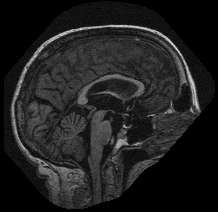
\includegraphics[width=1.014\textwidth]{images/1.png}
	\end{subfigure}
	\begin{subfigure}{.23\textwidth}
		\centering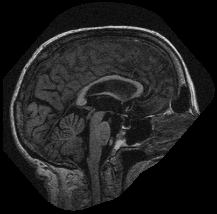
\includegraphics[width=\textwidth]{images/2.png}
	\end{subfigure}
	
	\begin{subfigure}{.23\textwidth}
		\centering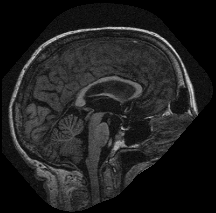
\includegraphics[width=1.013\textwidth]{images/3.png}
	\end{subfigure}
	\begin{subfigure}{.23\textwidth}
		\centering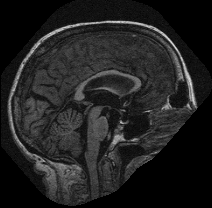
\includegraphics[width=\textwidth]{images/4.png}
	\end{subfigure}
	\caption{individual  T1-weighted  magnetization  prepared  rapid  gradient-echo  (MP-RAGE)  images of one random subject}
	\label{fig:1234}
\end{figure}


Averaged motion-corrected images are then produced using the T1-weighted MP-RAGE images for each subject to improve signal-to-noise ratio, which is shown in Figure \ref{fig:avg}.

\section{Data Preprocessing}

To retrieve volumetric information of different parts of the brain, we have to perform several preprocessing stages, a few of which are mentioned below:

\begin{itemize}
	\item Motion Correction and Conform
	\item NU (Non-Uniform intensity normalization)
	\item Talairach transform computation
	\item Intensity Normalization 1
	\item Skull Strip
	\item EM Register (linear volumetric registration)
	\item CA Intensity Normalization
	\item CA Non-linear Volumetric Registration
	\item Remove Neck
	\item LTA with Skull
	\item ...
\end{itemize}

\begin{figure}
	\centering
	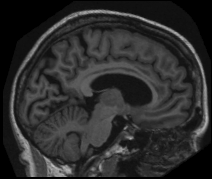
\includegraphics[width=0.4\textwidth]{images/avg.png}
	\caption{Averaged motion-corrected image of a random subject acquired from images in Figure \ref{fig:1234}}
	\label{fig:avg}
\end{figure} 

In total 31 preprocessing stages is performed on each image with the FreeSurfer image analysis suite, which is documented and freely available for download online (\href{http://surfer.nmr.mgh.harvard.edu/}{http://surfer.nmr.mgh.harvard.edu/}). Details of each step is described in detail in free-surfer documentation. The result of preprocessing is shown in Figure \ref{fig:pre} from sagittal, coronal, and transverse view. The preprocessed images are visualized using FSL tools which is a comprehensive library of analysis tools for FMRI, MRI and DTI brain imaging data. Figure \ref{fig:pre} shows how perfectly the skull is stripped, neck is totally removed, etc.

Out of 416 subjects MRI images, 199 images successfully preprocessed. Other images excluded from the dataset due to poor quality of the original image or unknown CDR label.

\begin{figure}
	\centering
	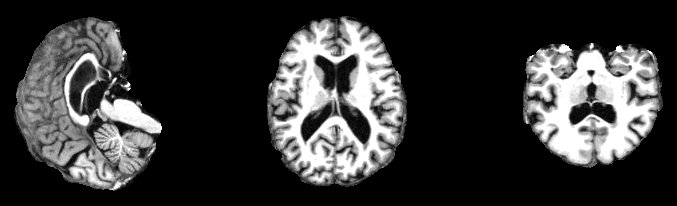
\includegraphics[width=\columnwidth]{images/preprocessed.png}
	\caption{Preprocessed image of the subject shown in Figure \ref{fig:avg} in sagittal, transverse, and coronal views (left to right)}
	\label{fig:pre}
\end{figure} 

\subsection{Feature Extraction}
Having preprocessed images, volume of different regions of the brain is extracted using the freesurfer tools. The features are obtained of brain segmentation and parcellation from both left and right hemisphere. 139 features related to the volume of different regions of interest are extracted in total, some of which are mentioned below:

\begin{enumerate}
	\item Left and right lateral ventricle
	\item Left and right cerebellum white matter
	\item Cerebrospinal fluid (CSF)
	\item Left and right hippocampus
	\item left and right hemisphere cortex
	\item Estimated total intra cranial (eTIV)
	\item left and right hemisphere surface holes
	\item ...
\end{enumerate}

Finally, as objective of the classification is to diagnose AD, the subjects with CDR greater than 0 are labeled as 1 (patient) and others (CDR = 0) are labeled as 0 (a control subject).

Table \ref{tab:dataset} shows the outline of the OASIS dataset.

\begin{table}
	\caption{OASIS Dataset}
	\label{tab:dataset}
	\centering
	\begin{tabular}{lp{4cm}}
		\hline 
		Classes & 2\\
		Samples total & 199 \\
		Samples per class & 86 (1), 113(0) \\
		Dimensionality & 139 \\
		Features & Real values \\ \hline
	\end{tabular}
\end{table}


%\section{Visualization}
%
%Visualization is done in 2 stages:
%\begin{enumerate}
%	\item Importing Data with \texttt{Pandas} python library.
%	\item Exploring Data through Visualizations with Matplotlib
%\end{enumerate}
%
%

%\subsection{Feature Selection}
%
%Tree-based estimators can be used to compute feature importances, which in turn can be used to discard irrelevant features.
%
%Using feature importances with random forest classification, we can draw the importance of features to see if feature selection is necessary or not. The importance of features received from Random Forest model is shown in Figure.

\section{Visualization}

The dataset is almost a balanced dataset, i.e. the number of samples of patients and controlled subjects is balanced. Figure \ref{fig:dataset-balance} shows the dataset balance. 
\begin{figure}
	\centering
	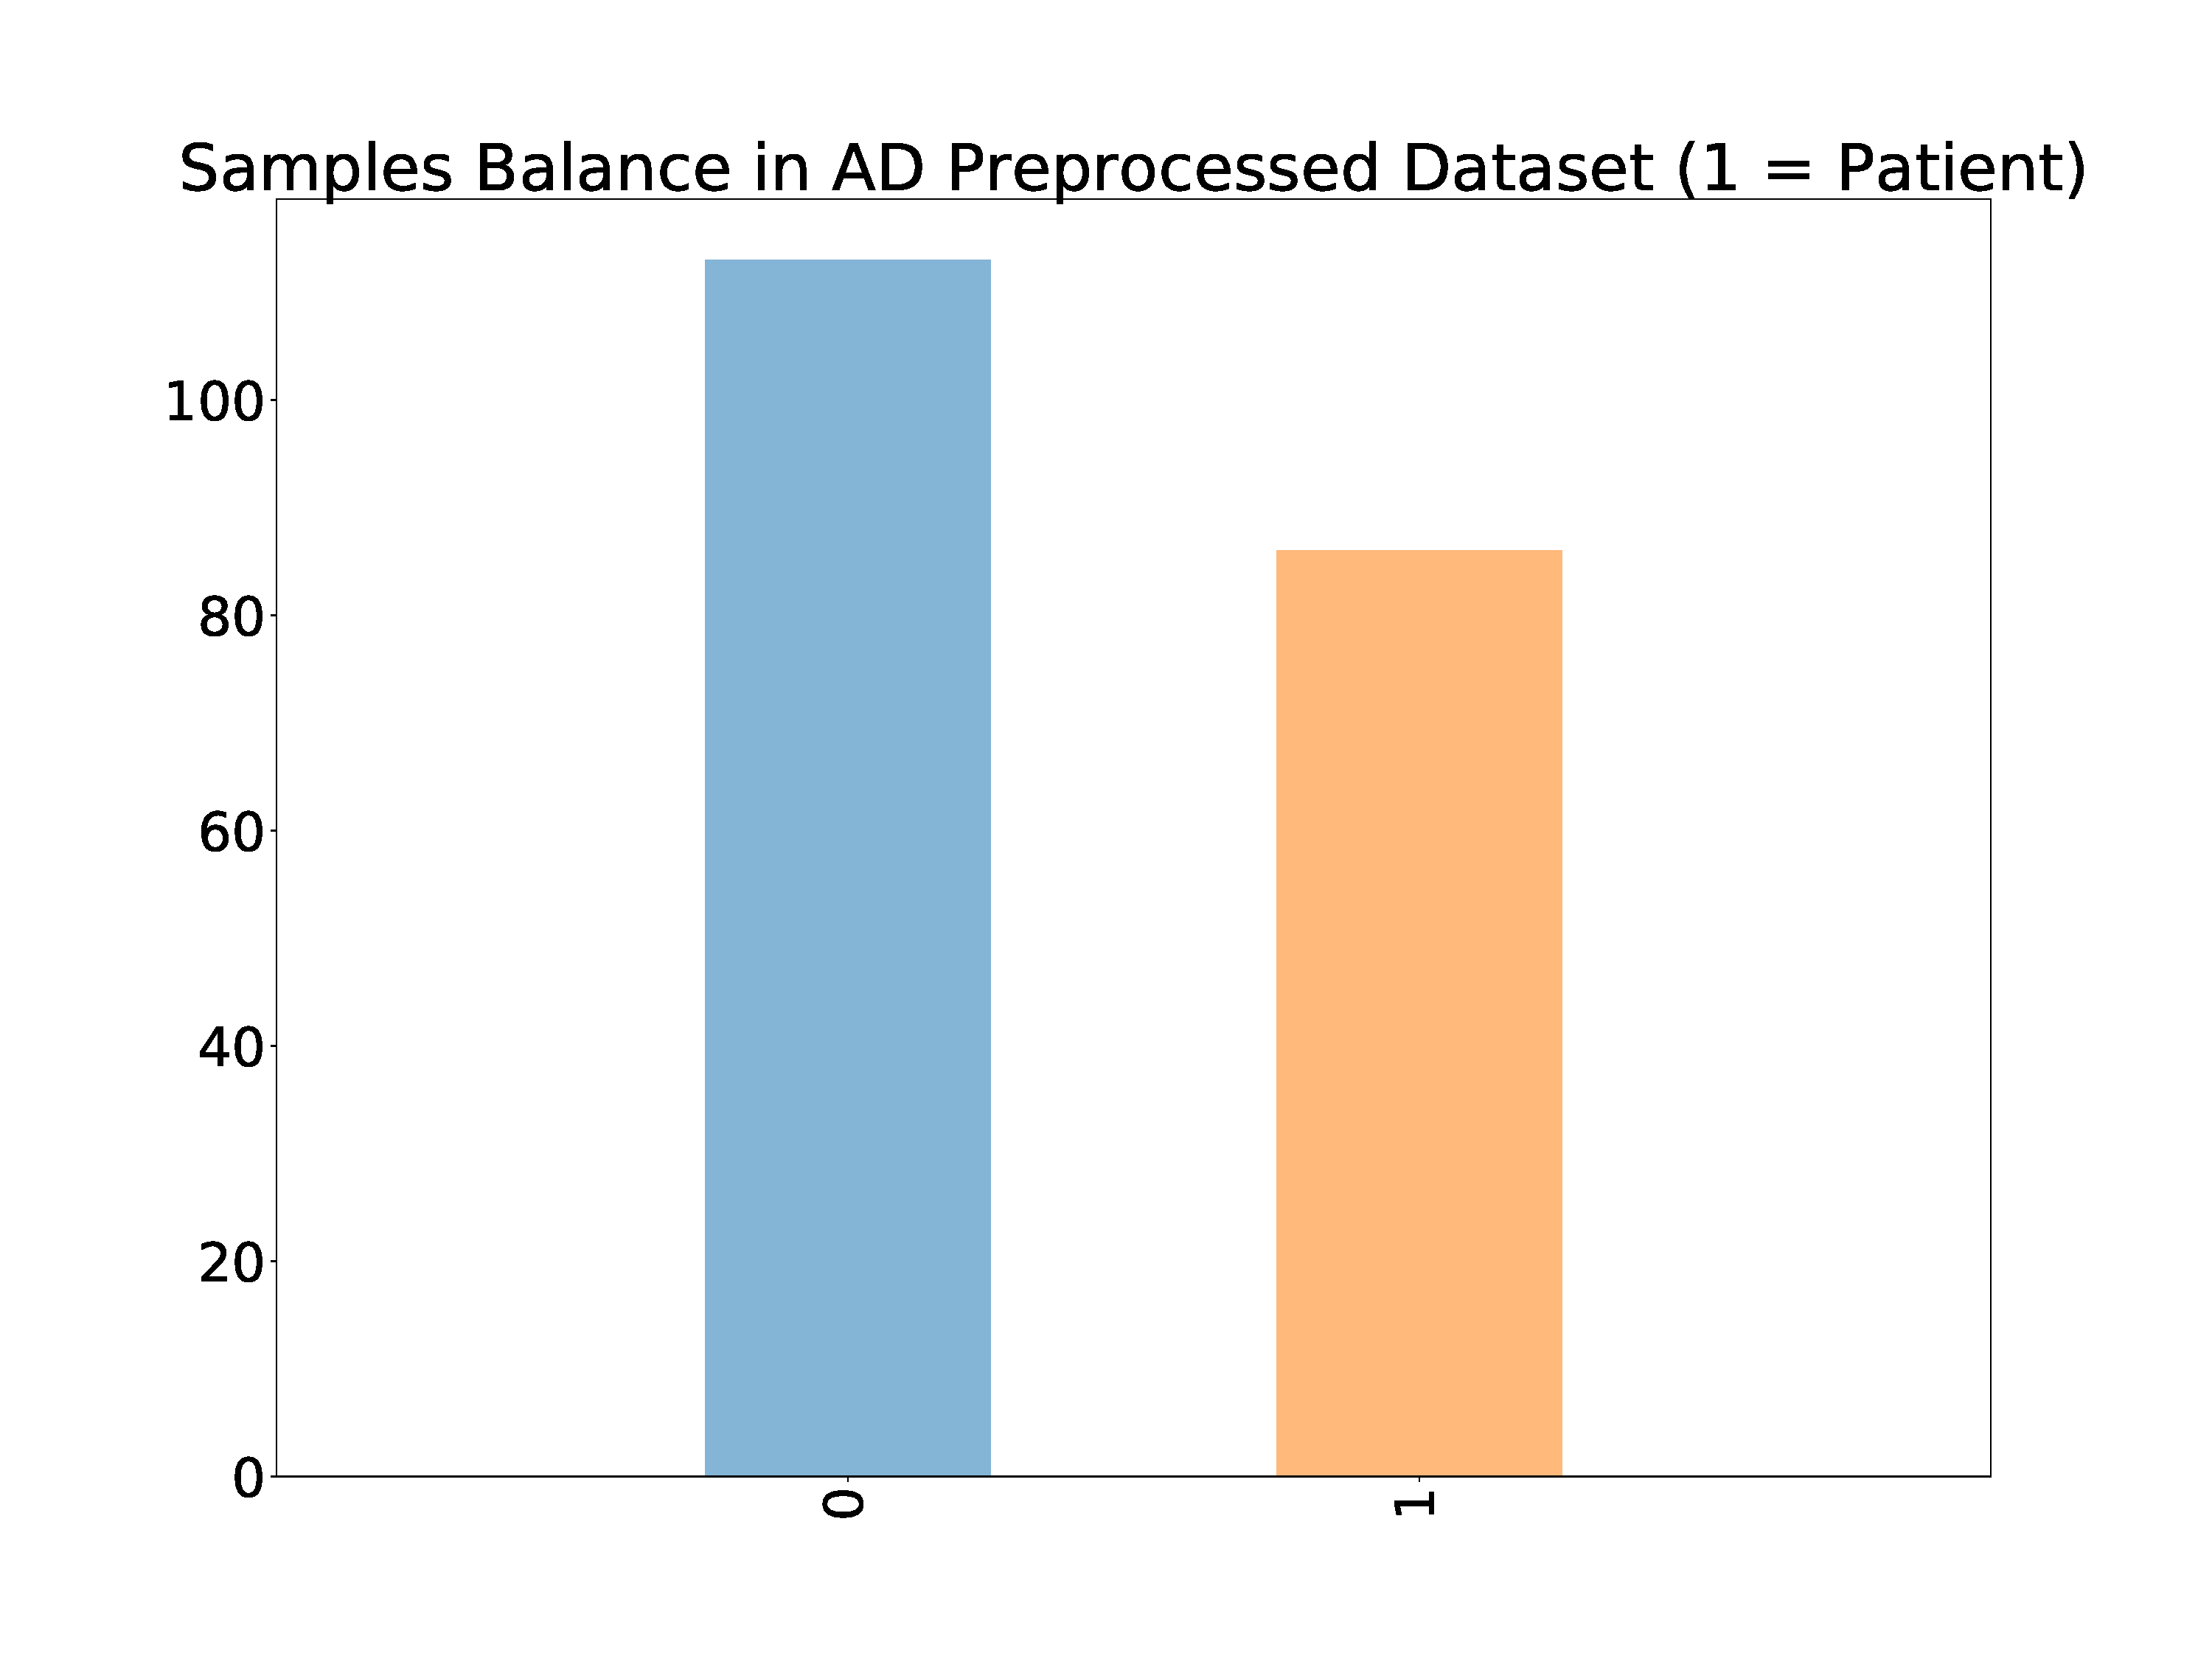
\includegraphics[width=\columnwidth]{images/dataset-balance.pdf}
	\caption{Dataset balance}
	\label{fig:dataset-balance}
\end{figure} 

The greatest known risk factor for Alzheimer’s is increasing age. Most individuals with the disease are 65 and older. This is shown in Figure \ref{fig:AD-distribution-age} as the distribution of age in the dataset for patients and controlled subjects.

\begin{figure}
	\centering
	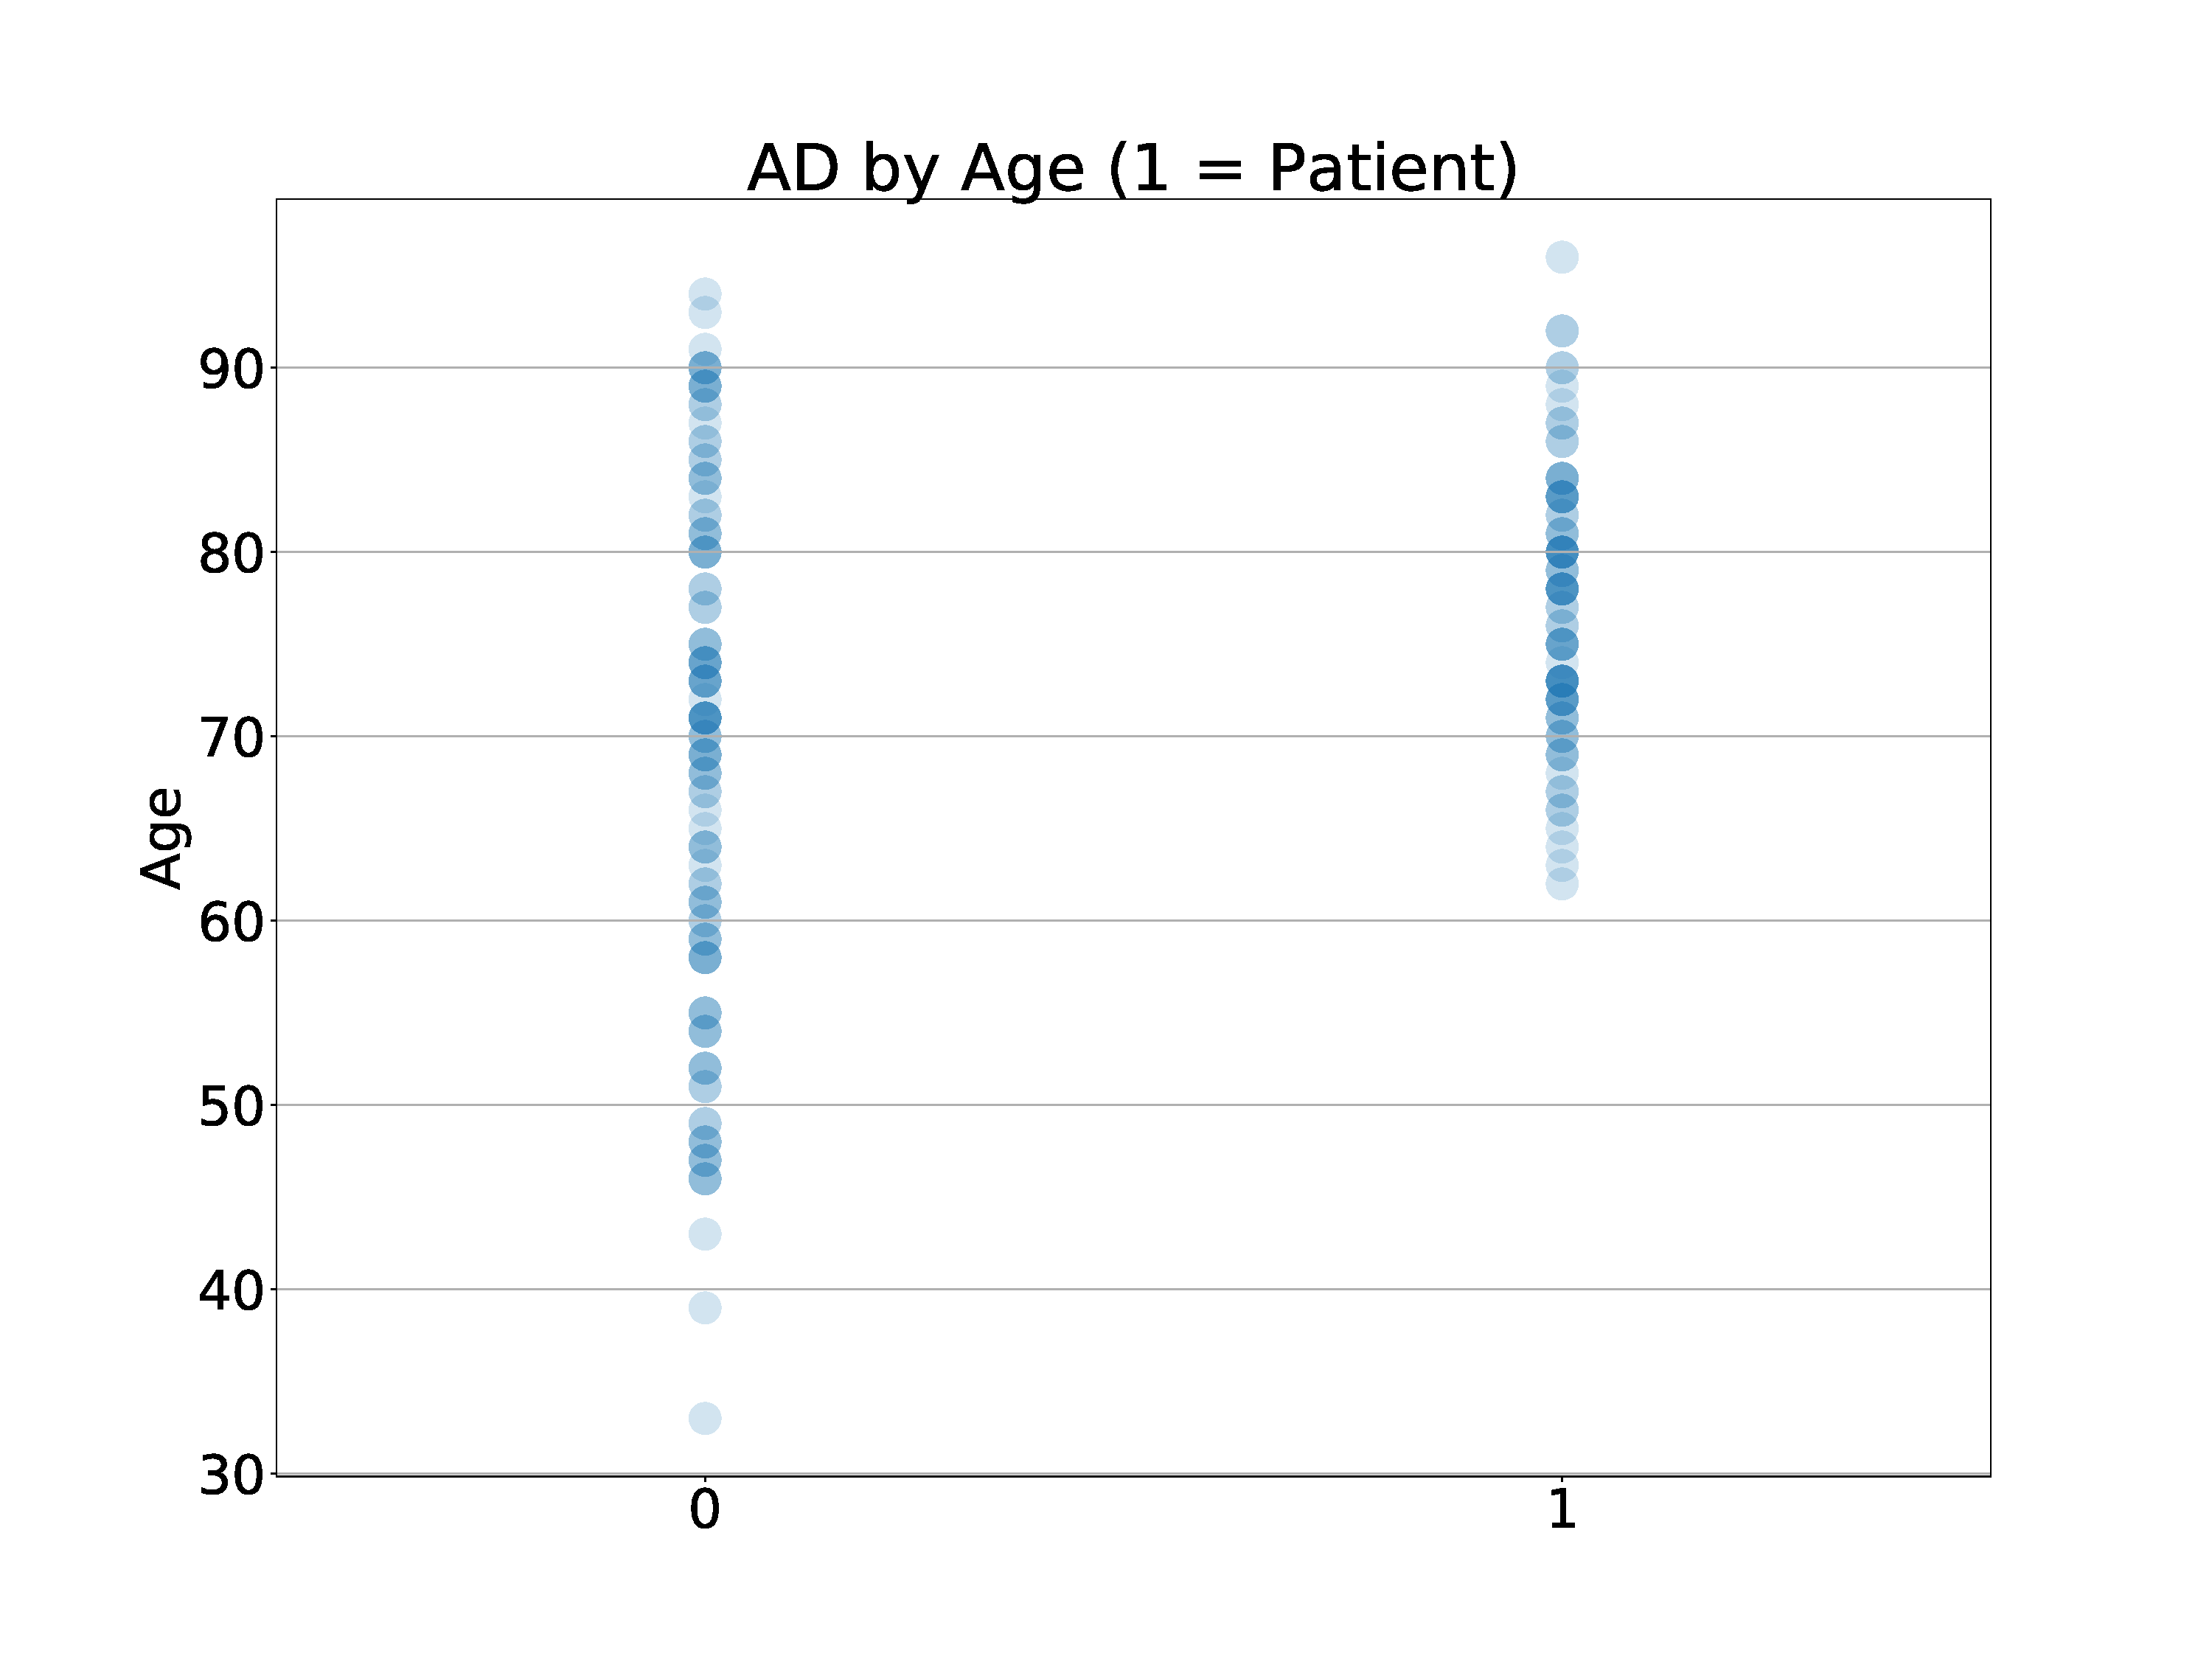
\includegraphics[width=\columnwidth]{images/AD-distribution-age.pdf}
	\caption{Distribution of AD with age}
	\label{fig:AD-distribution-age}
\end{figure} 

As AD progresses, brain tissue shrinks. As an example, the brain mask volume and eTIV features extracted after preprocessing are shown in Figures \ref{fig:AD-MaskVol} and \ref{fig:AD-eTIV}, respectively. It can be seen from the figures that patients are likely to have smaller eTIV and brain mask which can be effectively used in identification of AD.

\begin{figure}
	\centering
	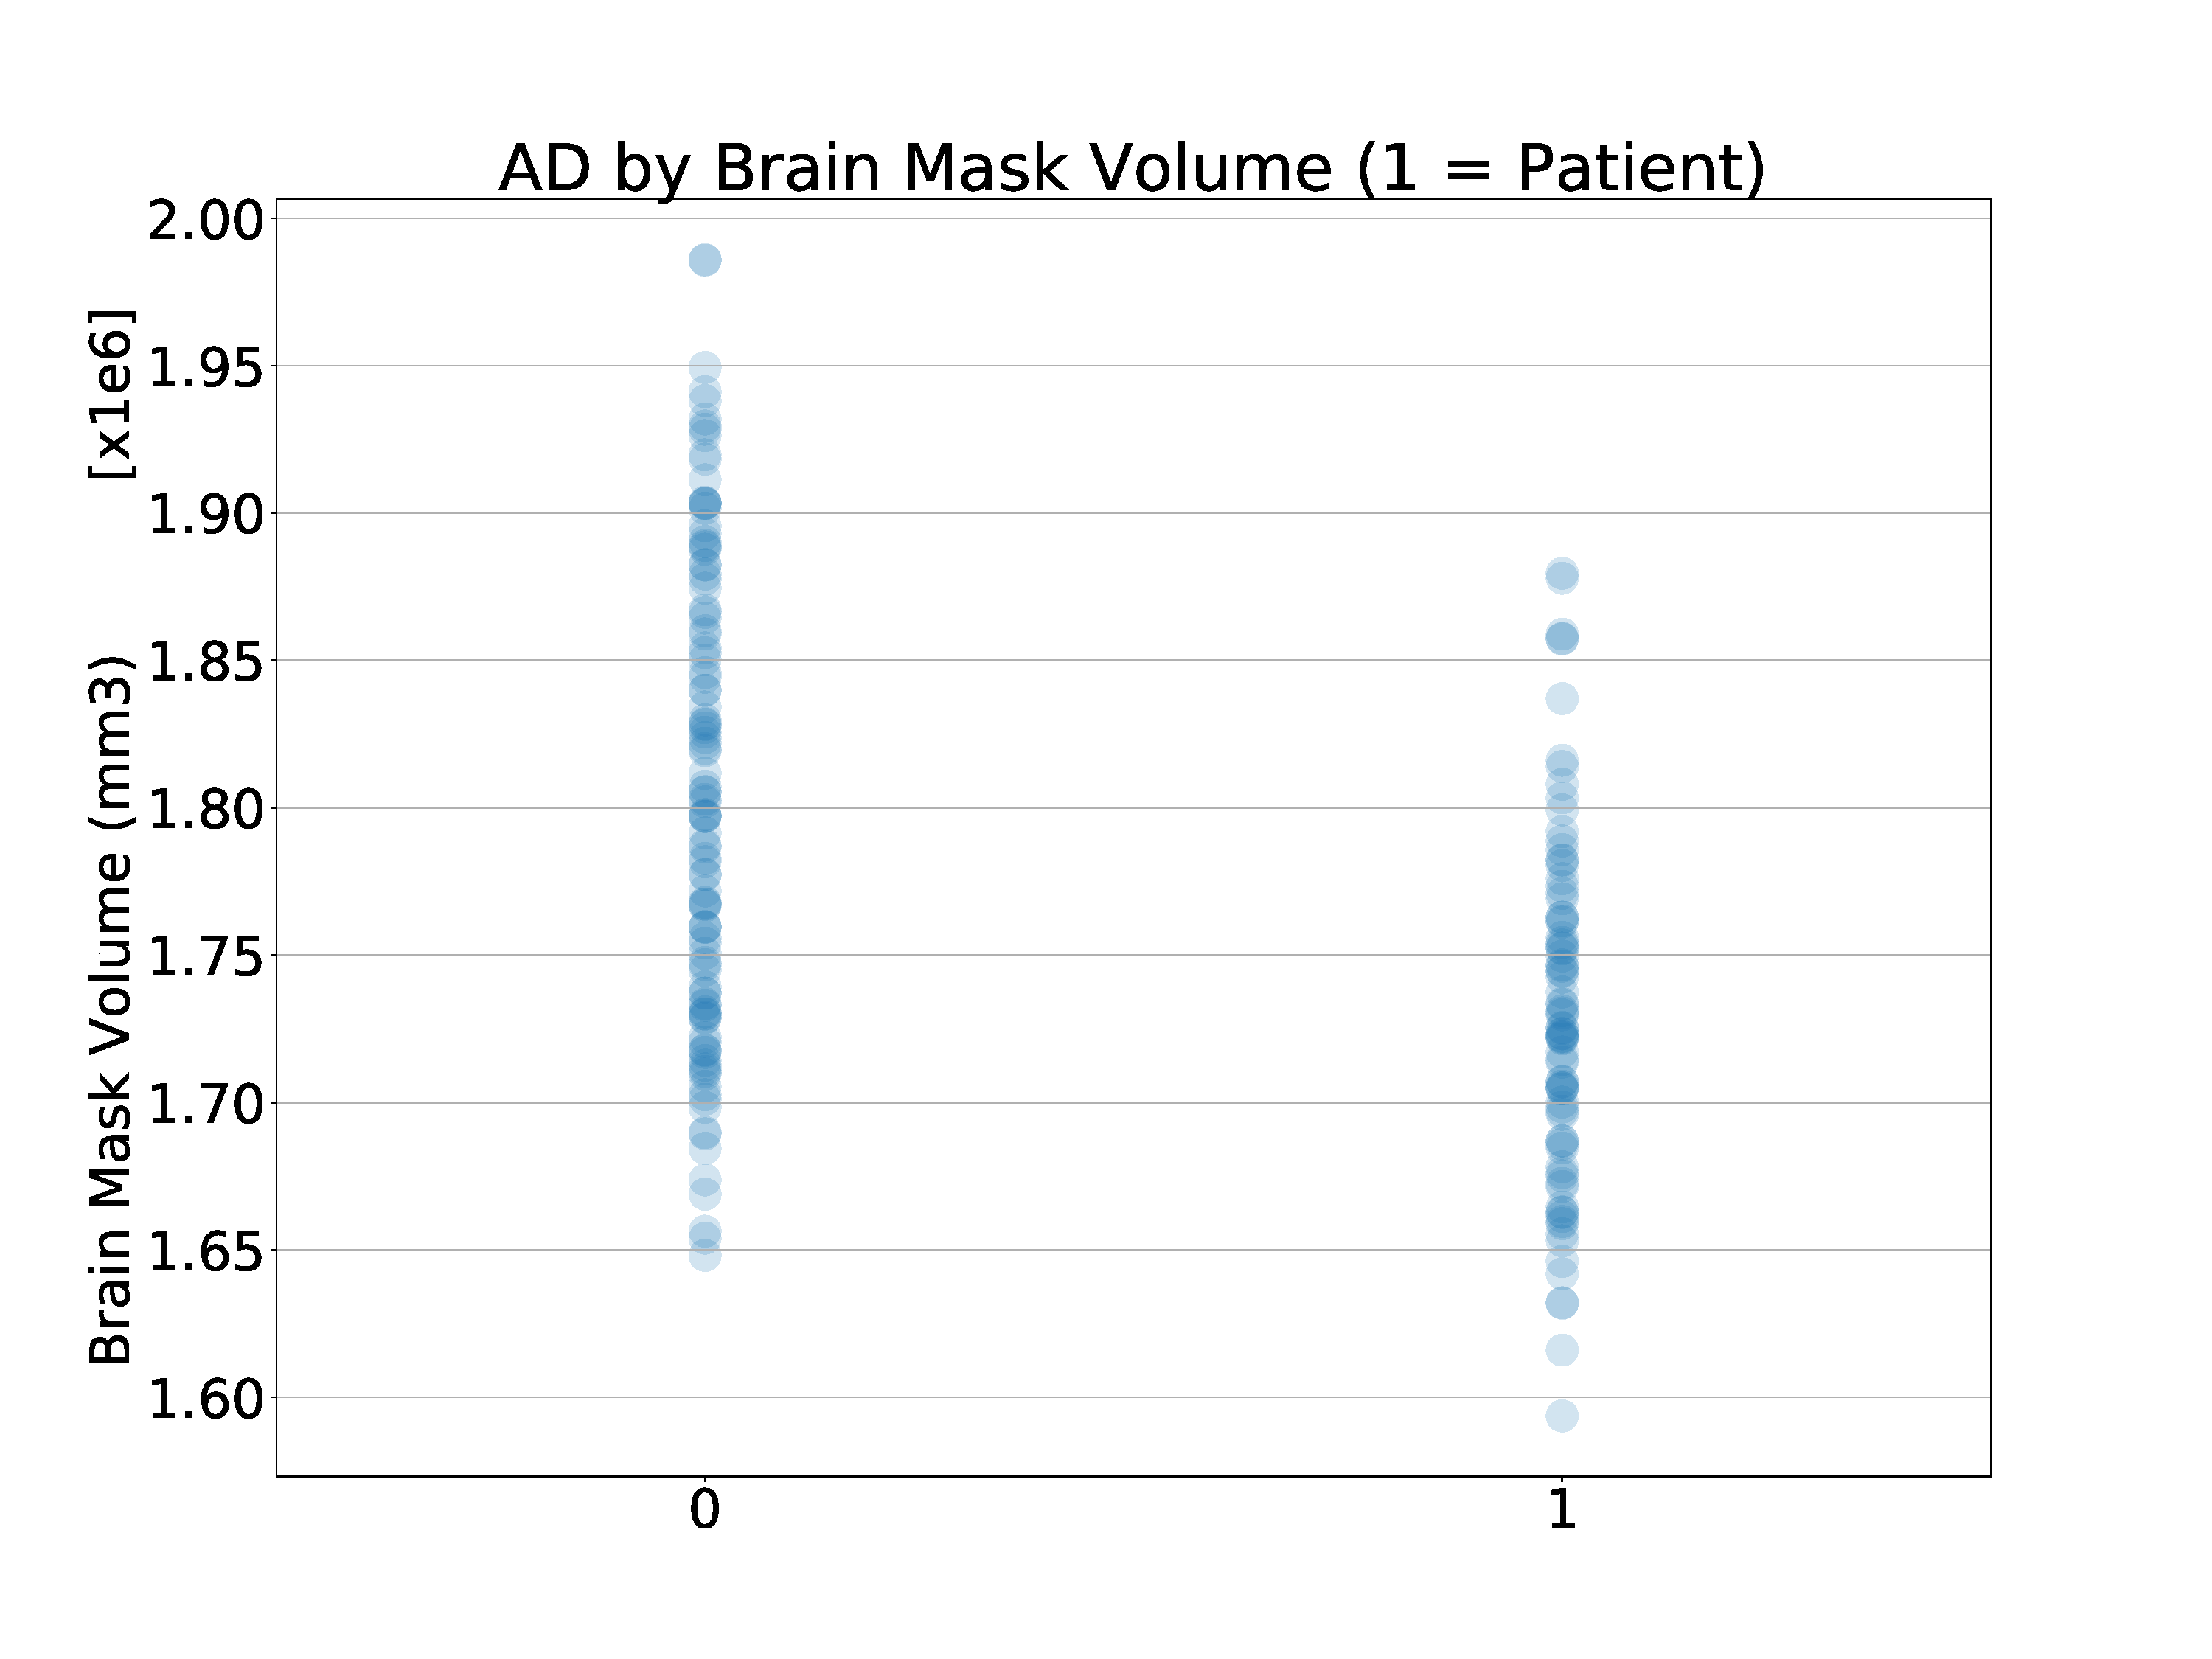
\includegraphics[width=\columnwidth]{images/AD-MaskVol.pdf}
	\caption{Brain mask shrinkage in AD patients and contorlled subjects}
	\label{fig:AD-MaskVol}
\end{figure} 

\begin{figure}
	\centering
	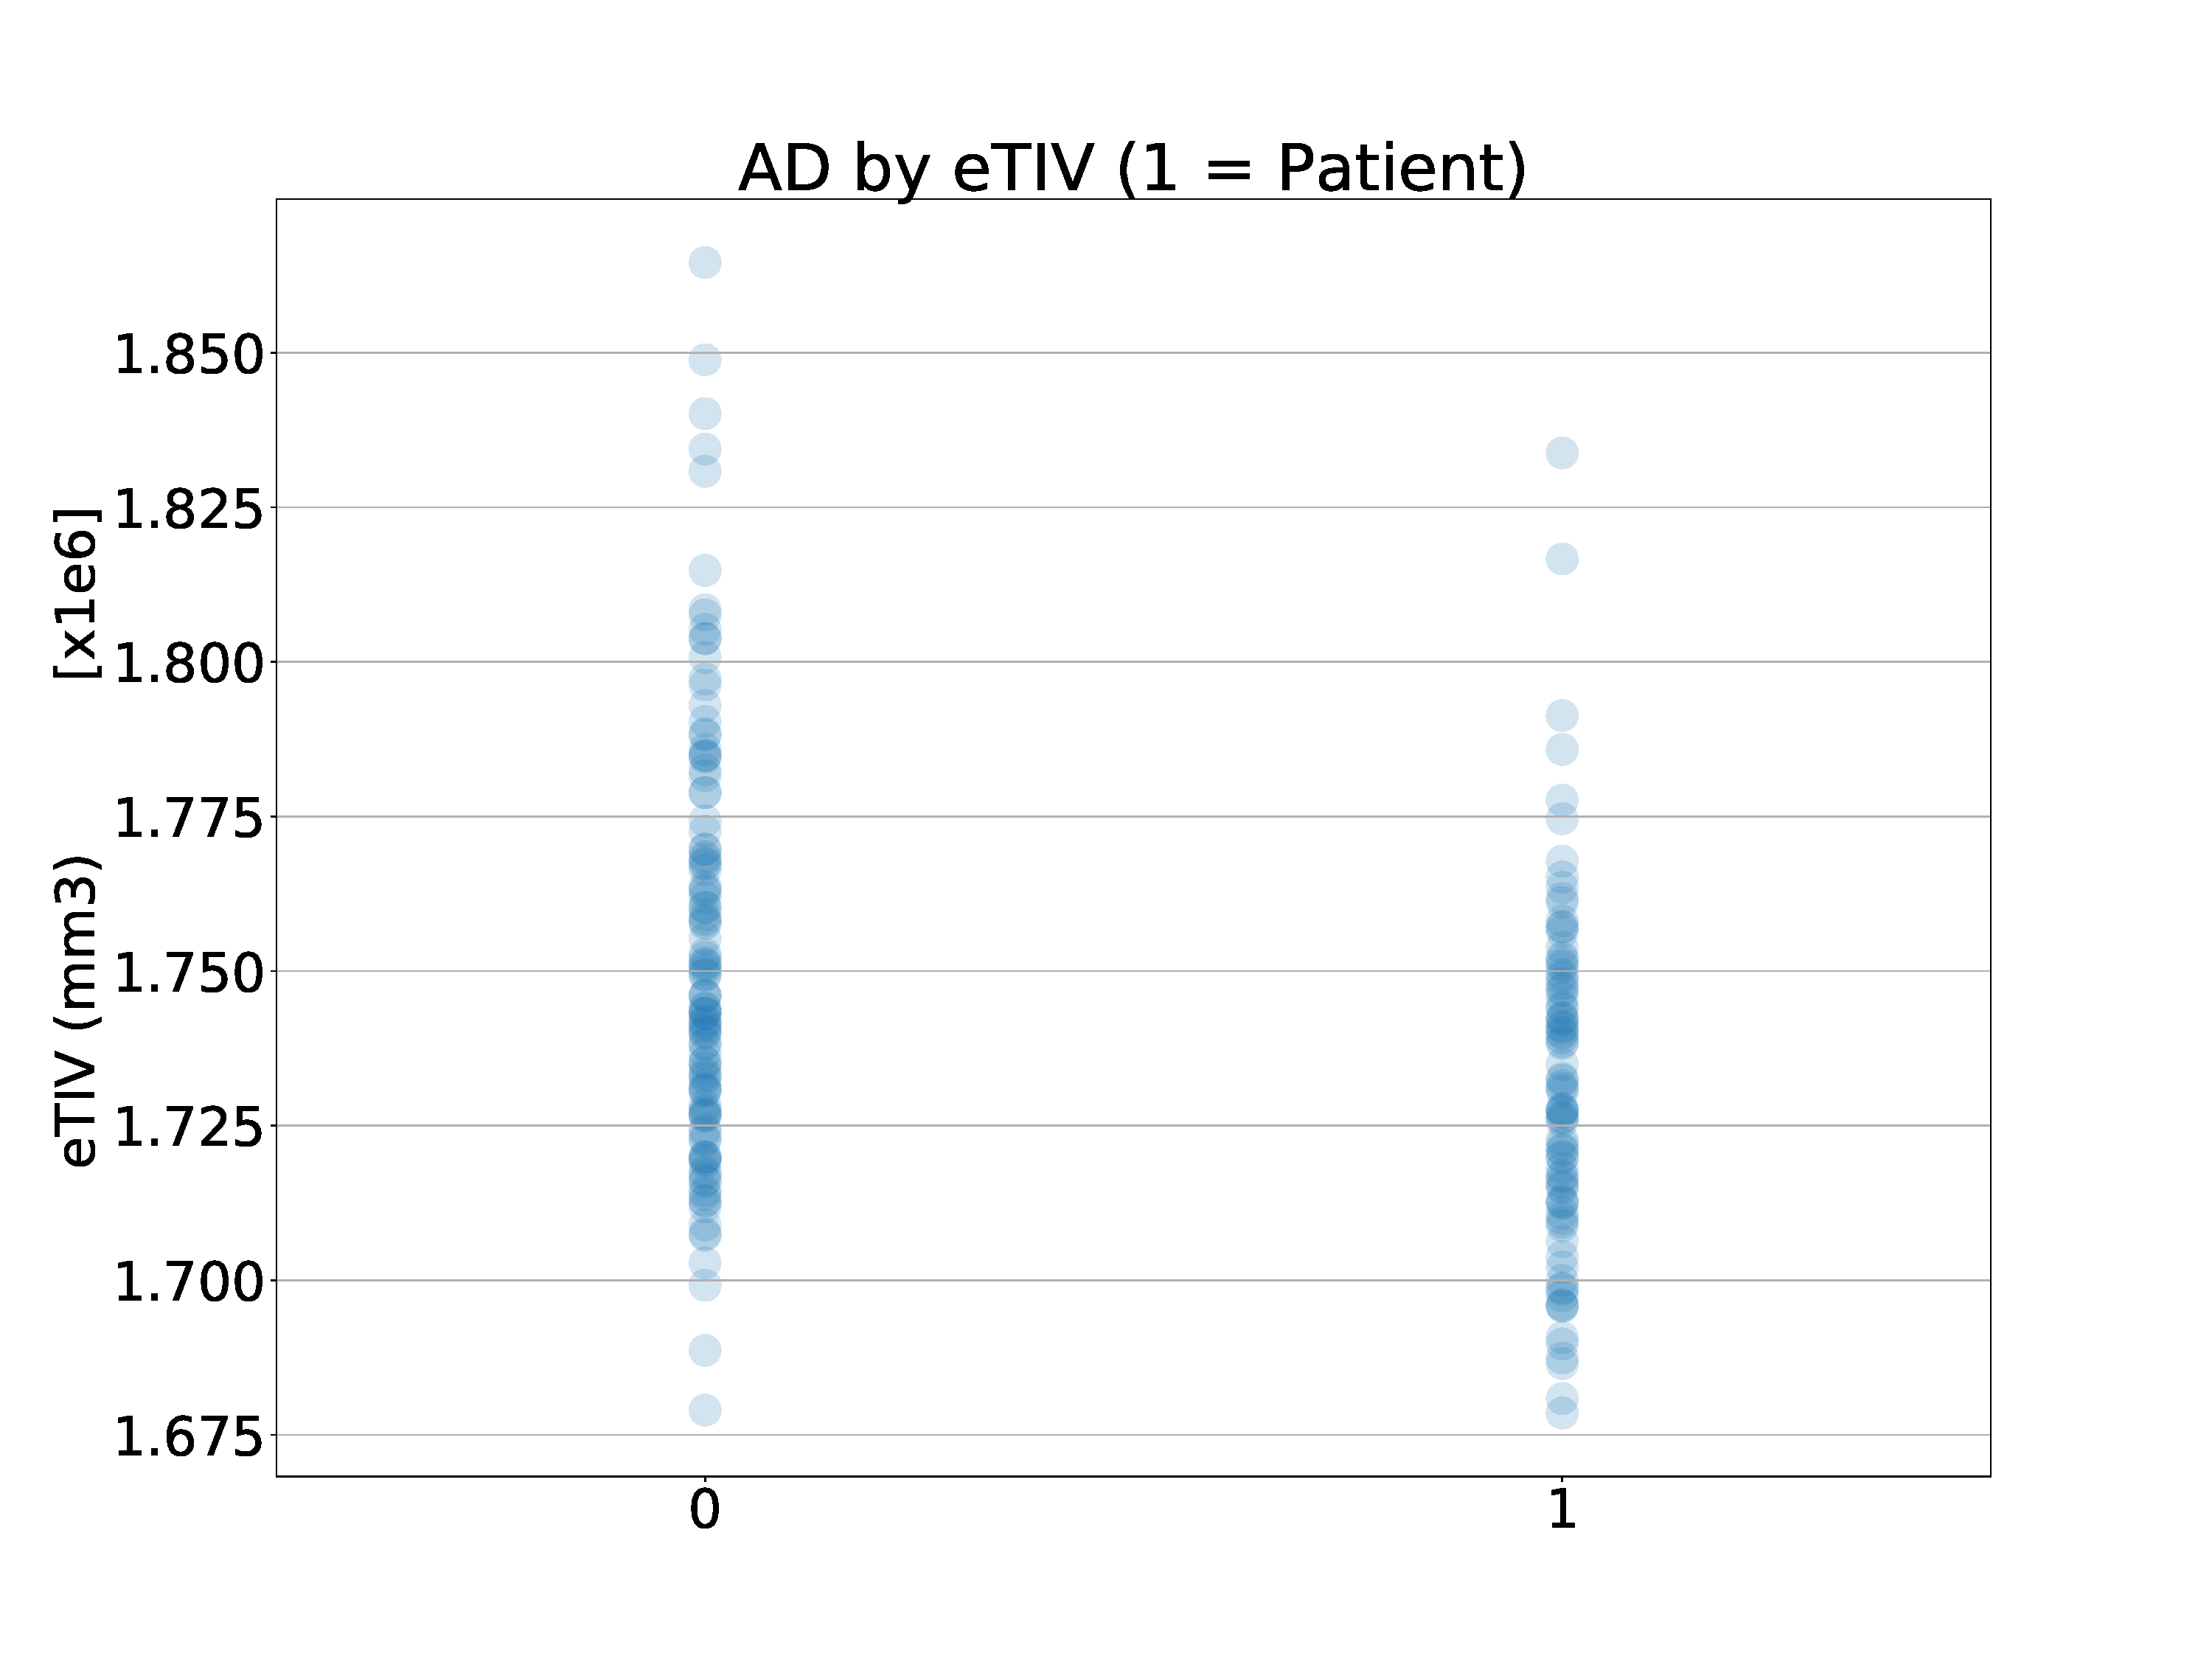
\includegraphics[width=\columnwidth]{images/AD-eTIV.pdf}
	\caption{eTIV shrinkage in AD patients and contorlled subjects}
	\label{fig:AD-eTIV}
\end{figure} 

As another example, cerebral white matter and cortex volume are shown in Figures \ref{fig:AD-WhiteMatter} and \ref{fig:AD-CortexVol}, respectively. The figure shown that the two features tend to have smaller value in patient compared to controlled subjects. If we use both features, it helps more to make patients separable from controlled subjects. This is shown in Figure \ref{fig:AD-Age-CortexVol-WhiteMatter}. Compared to the individual cerebral white matter by age and cortex volume by age, patients and controlled subjects are more separable. Therefore, classification by using all the 139 volumetric features extracted after preprocessing helps to achieve a high accuracy in AD identification.

\begin{figure}
	\centering
	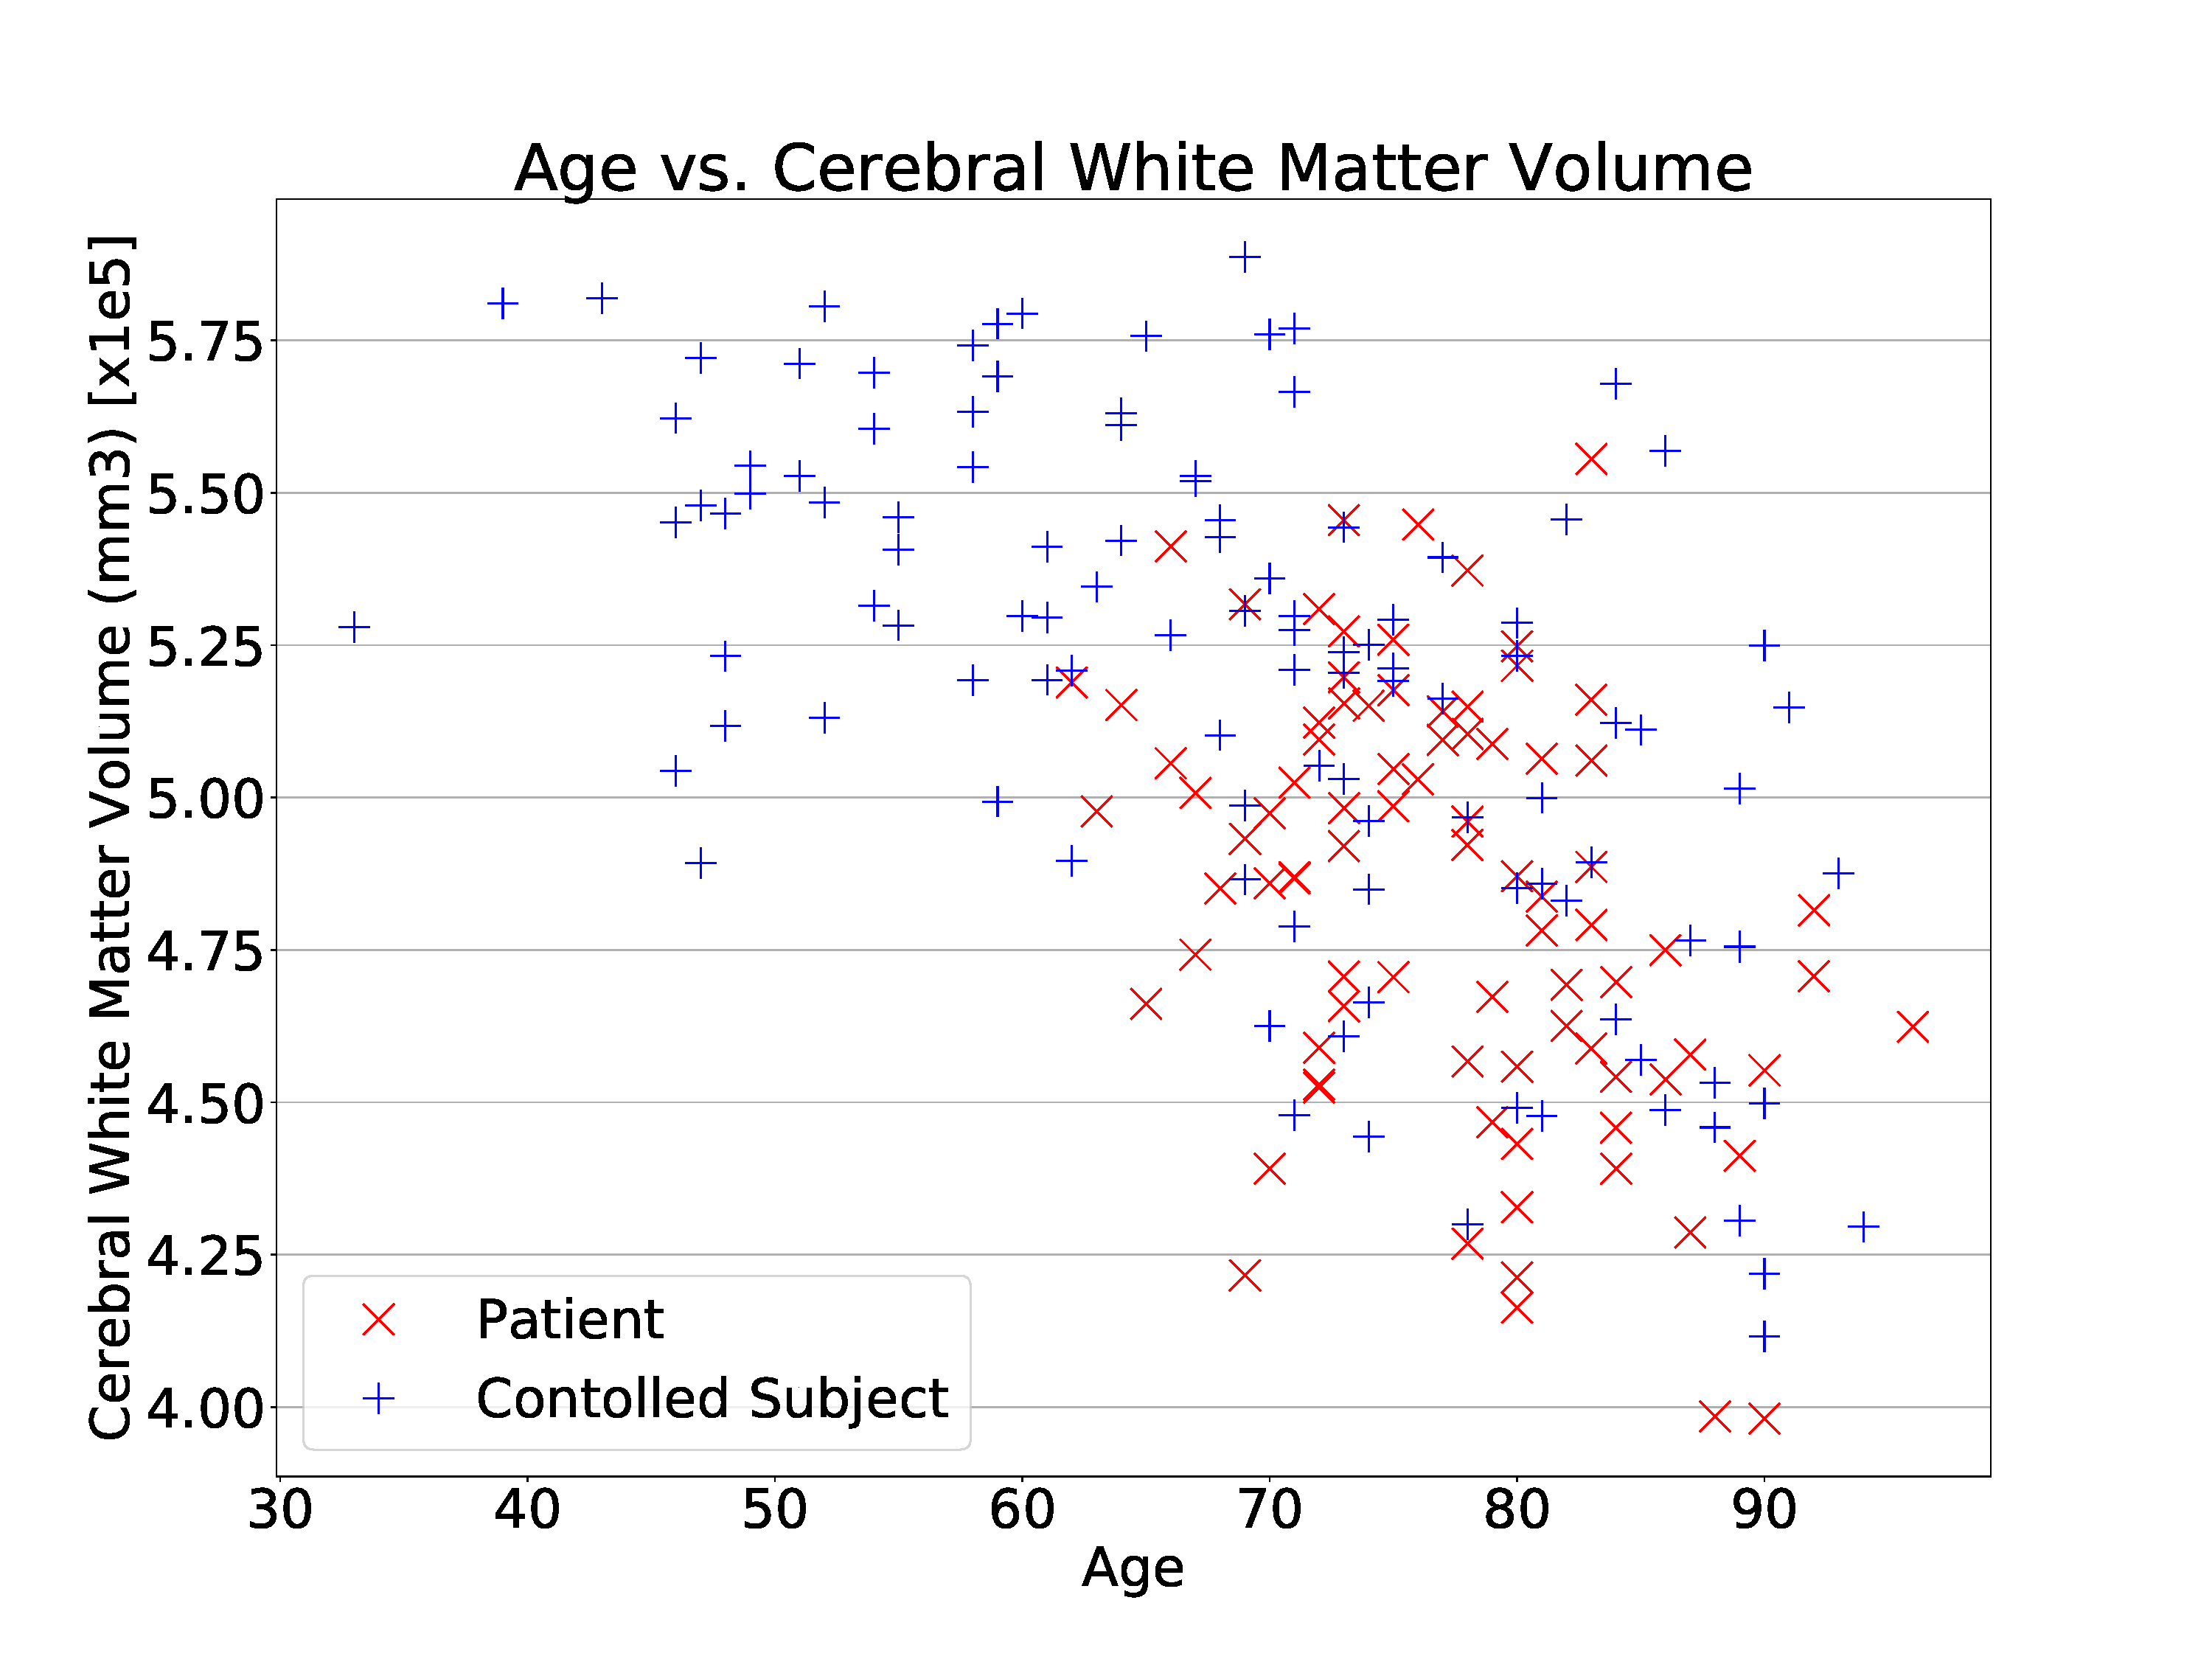
\includegraphics[width=\columnwidth]{images/AD-Age-WhiteMatter.pdf}
	\caption{AD relation with cerebral white matter volume and age}
	\label{fig:AD-WhiteMatter}
\end{figure} 

\begin{figure}
	\centering
	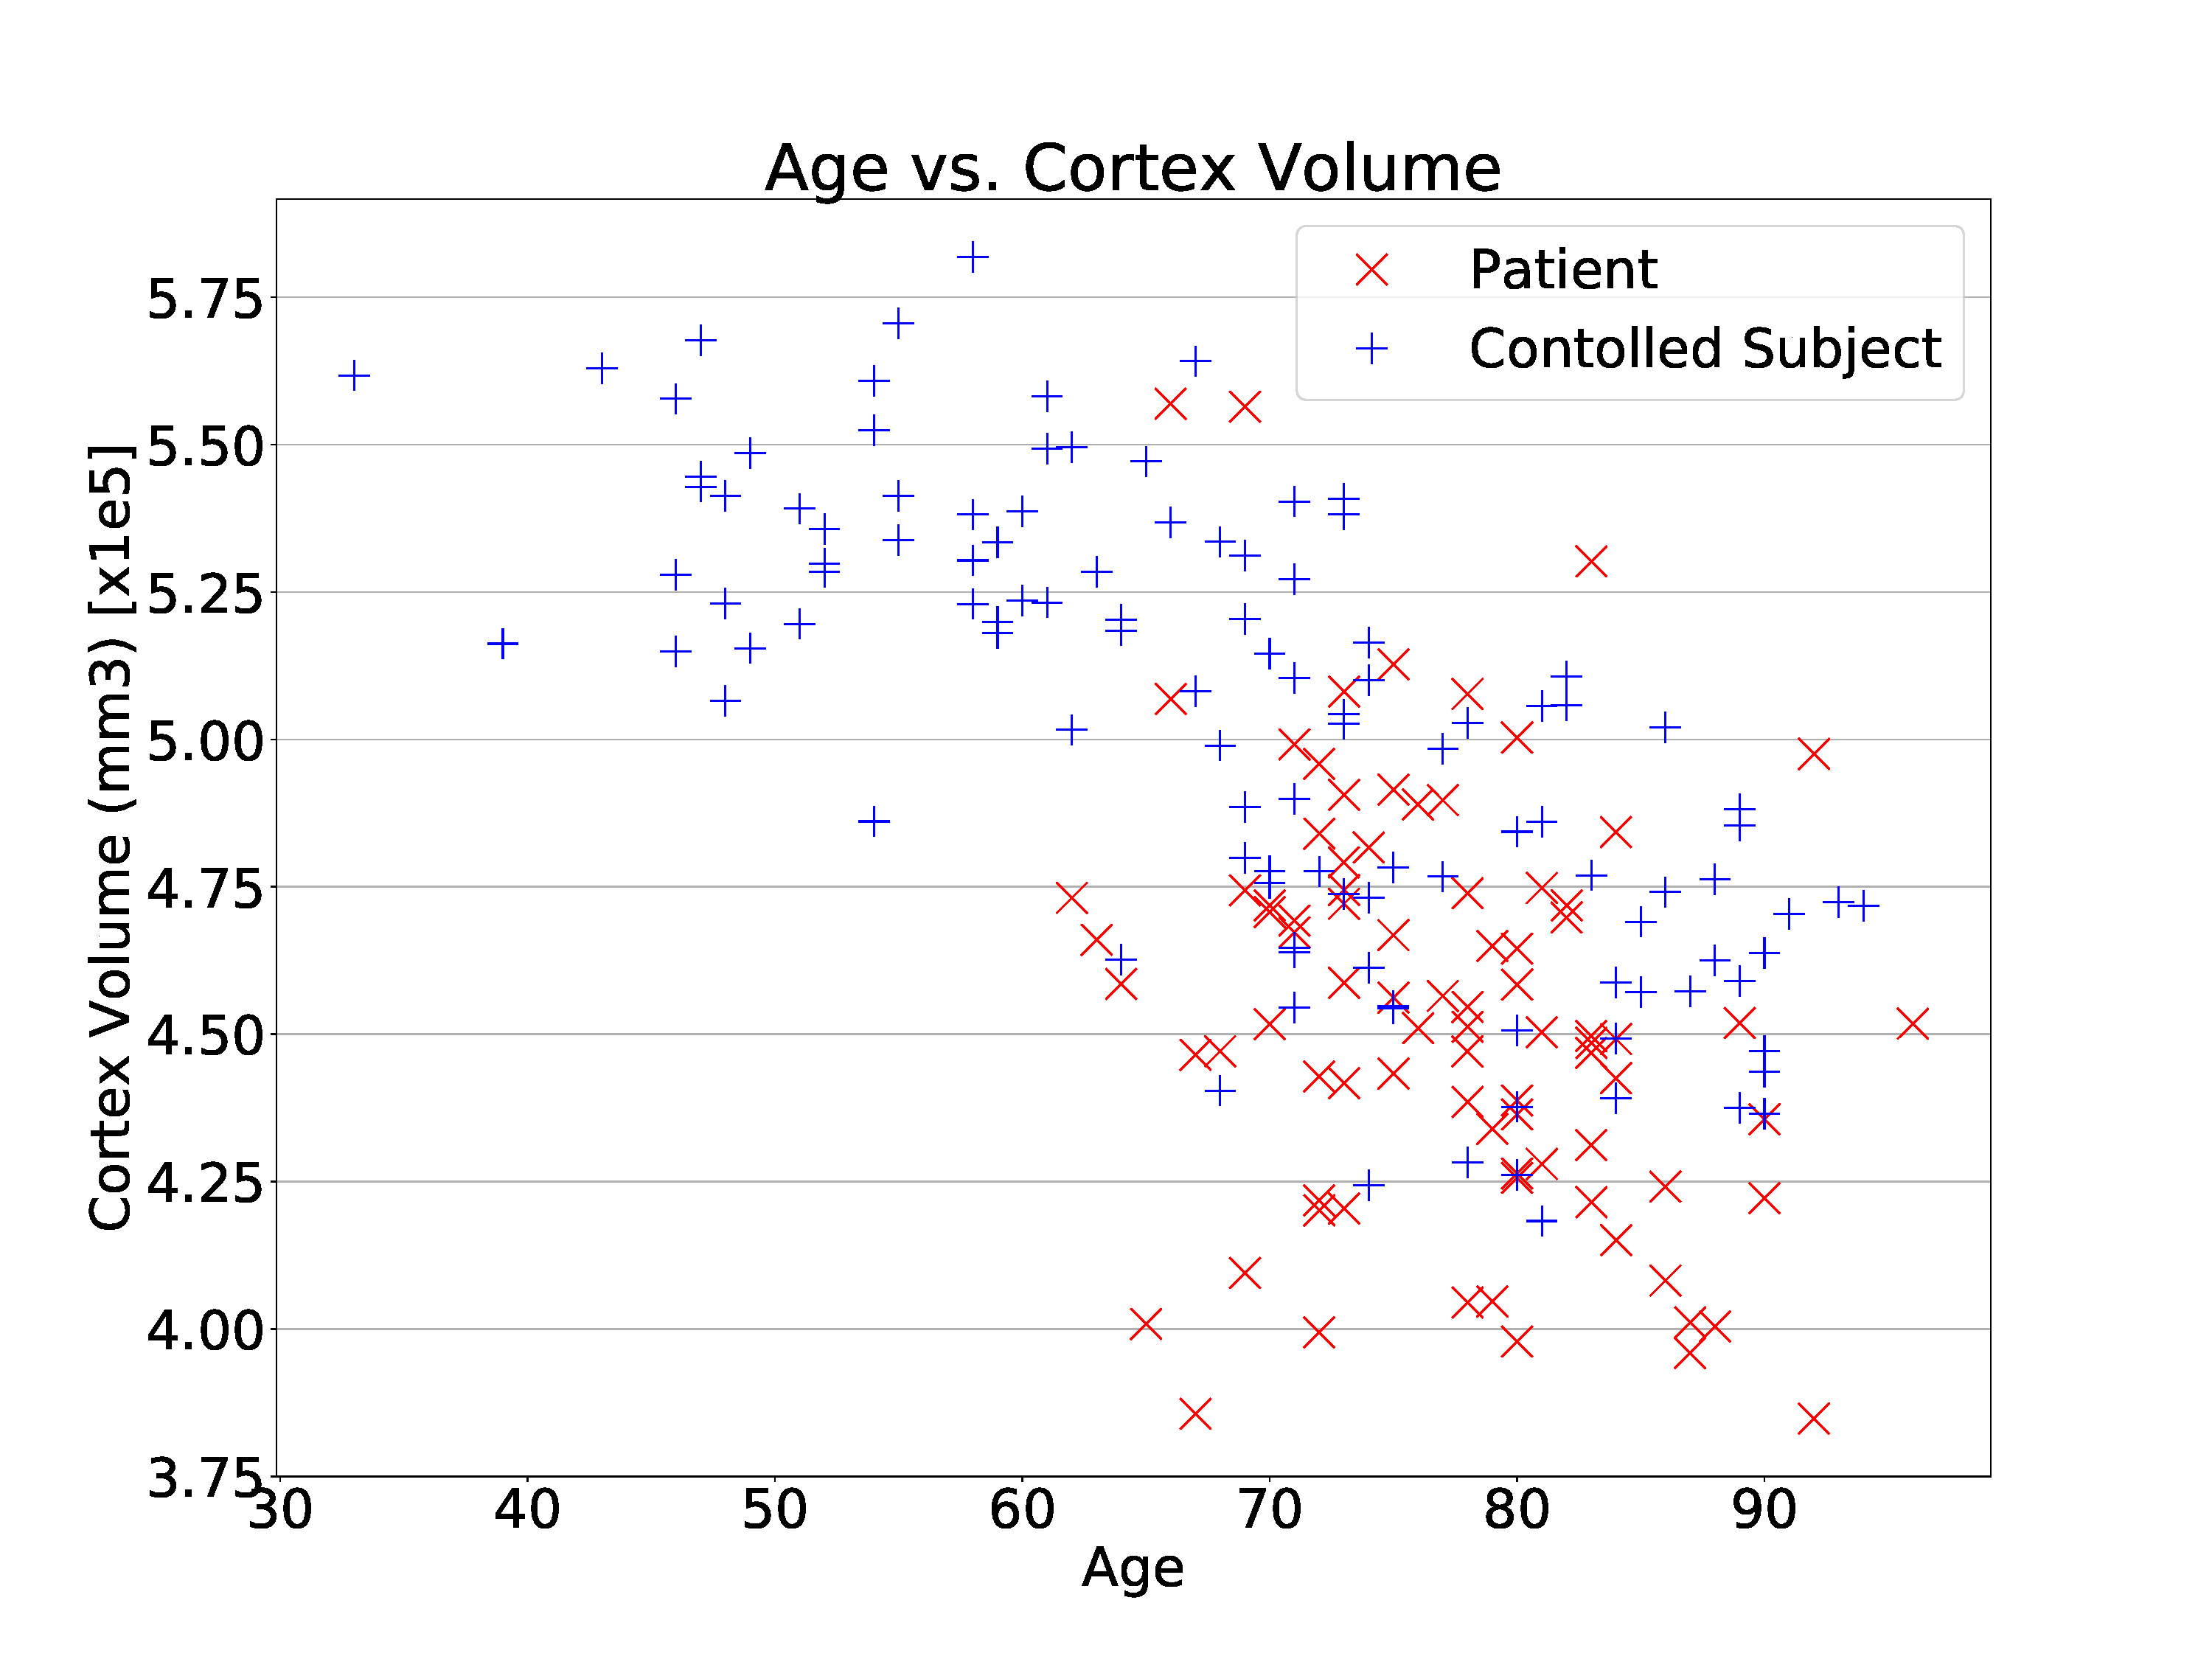
\includegraphics[width=\columnwidth]{images/AD-Age-CortexVol.pdf}
	\caption{AD relation with cortex volume and age}
	\label{fig:AD-CortexVol}
\end{figure}



\begin{figure}
	\centering
	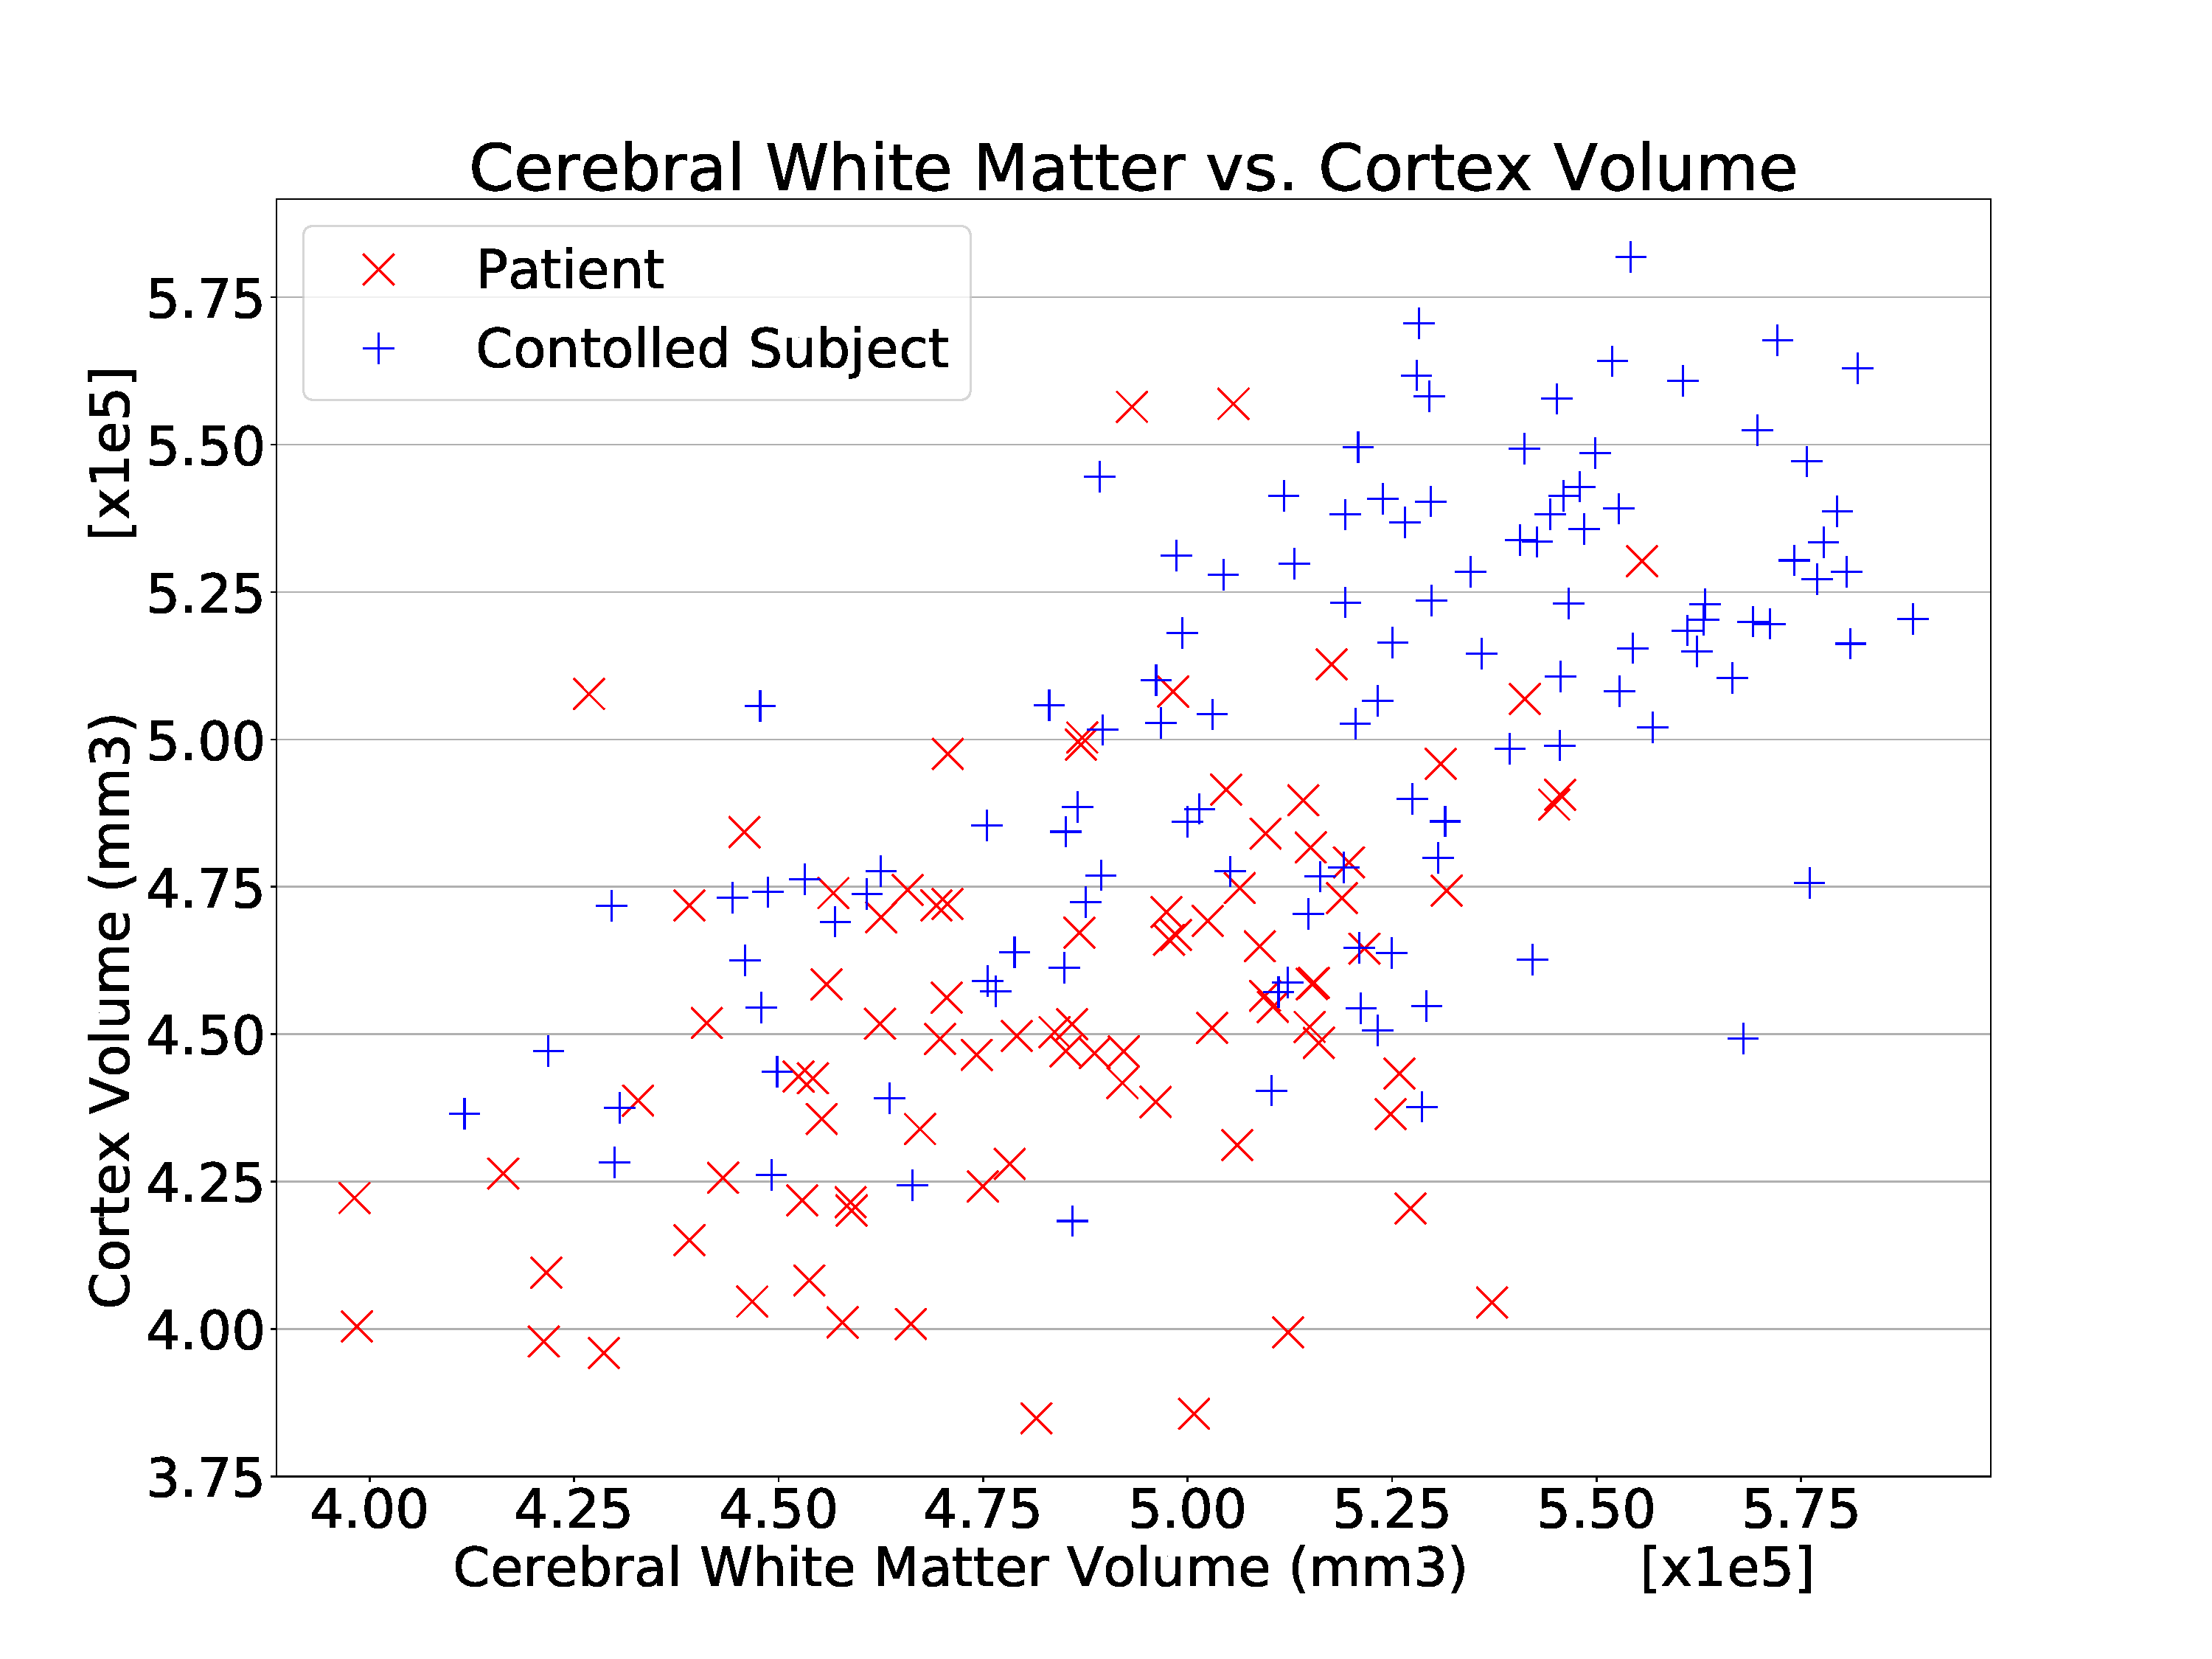
\includegraphics[width=\columnwidth]{images/AD-CWMVolCortexVol.pdf}
	\caption{Cerebral white matter volume vs. cortex volume in AD patients and controlled subjects}
	\label{fig:AD-Age-CortexVol-WhiteMatter}
\end{figure}

In contrast, the ventricles, chambers within the brain that contain CSF, are noticeably enlarged in AD patients. This is shown in Figure \ref{fig:AD-Age-CSF.pdf} by plotting the CSF volume versus age.  

\begin{figure}
	\centering
	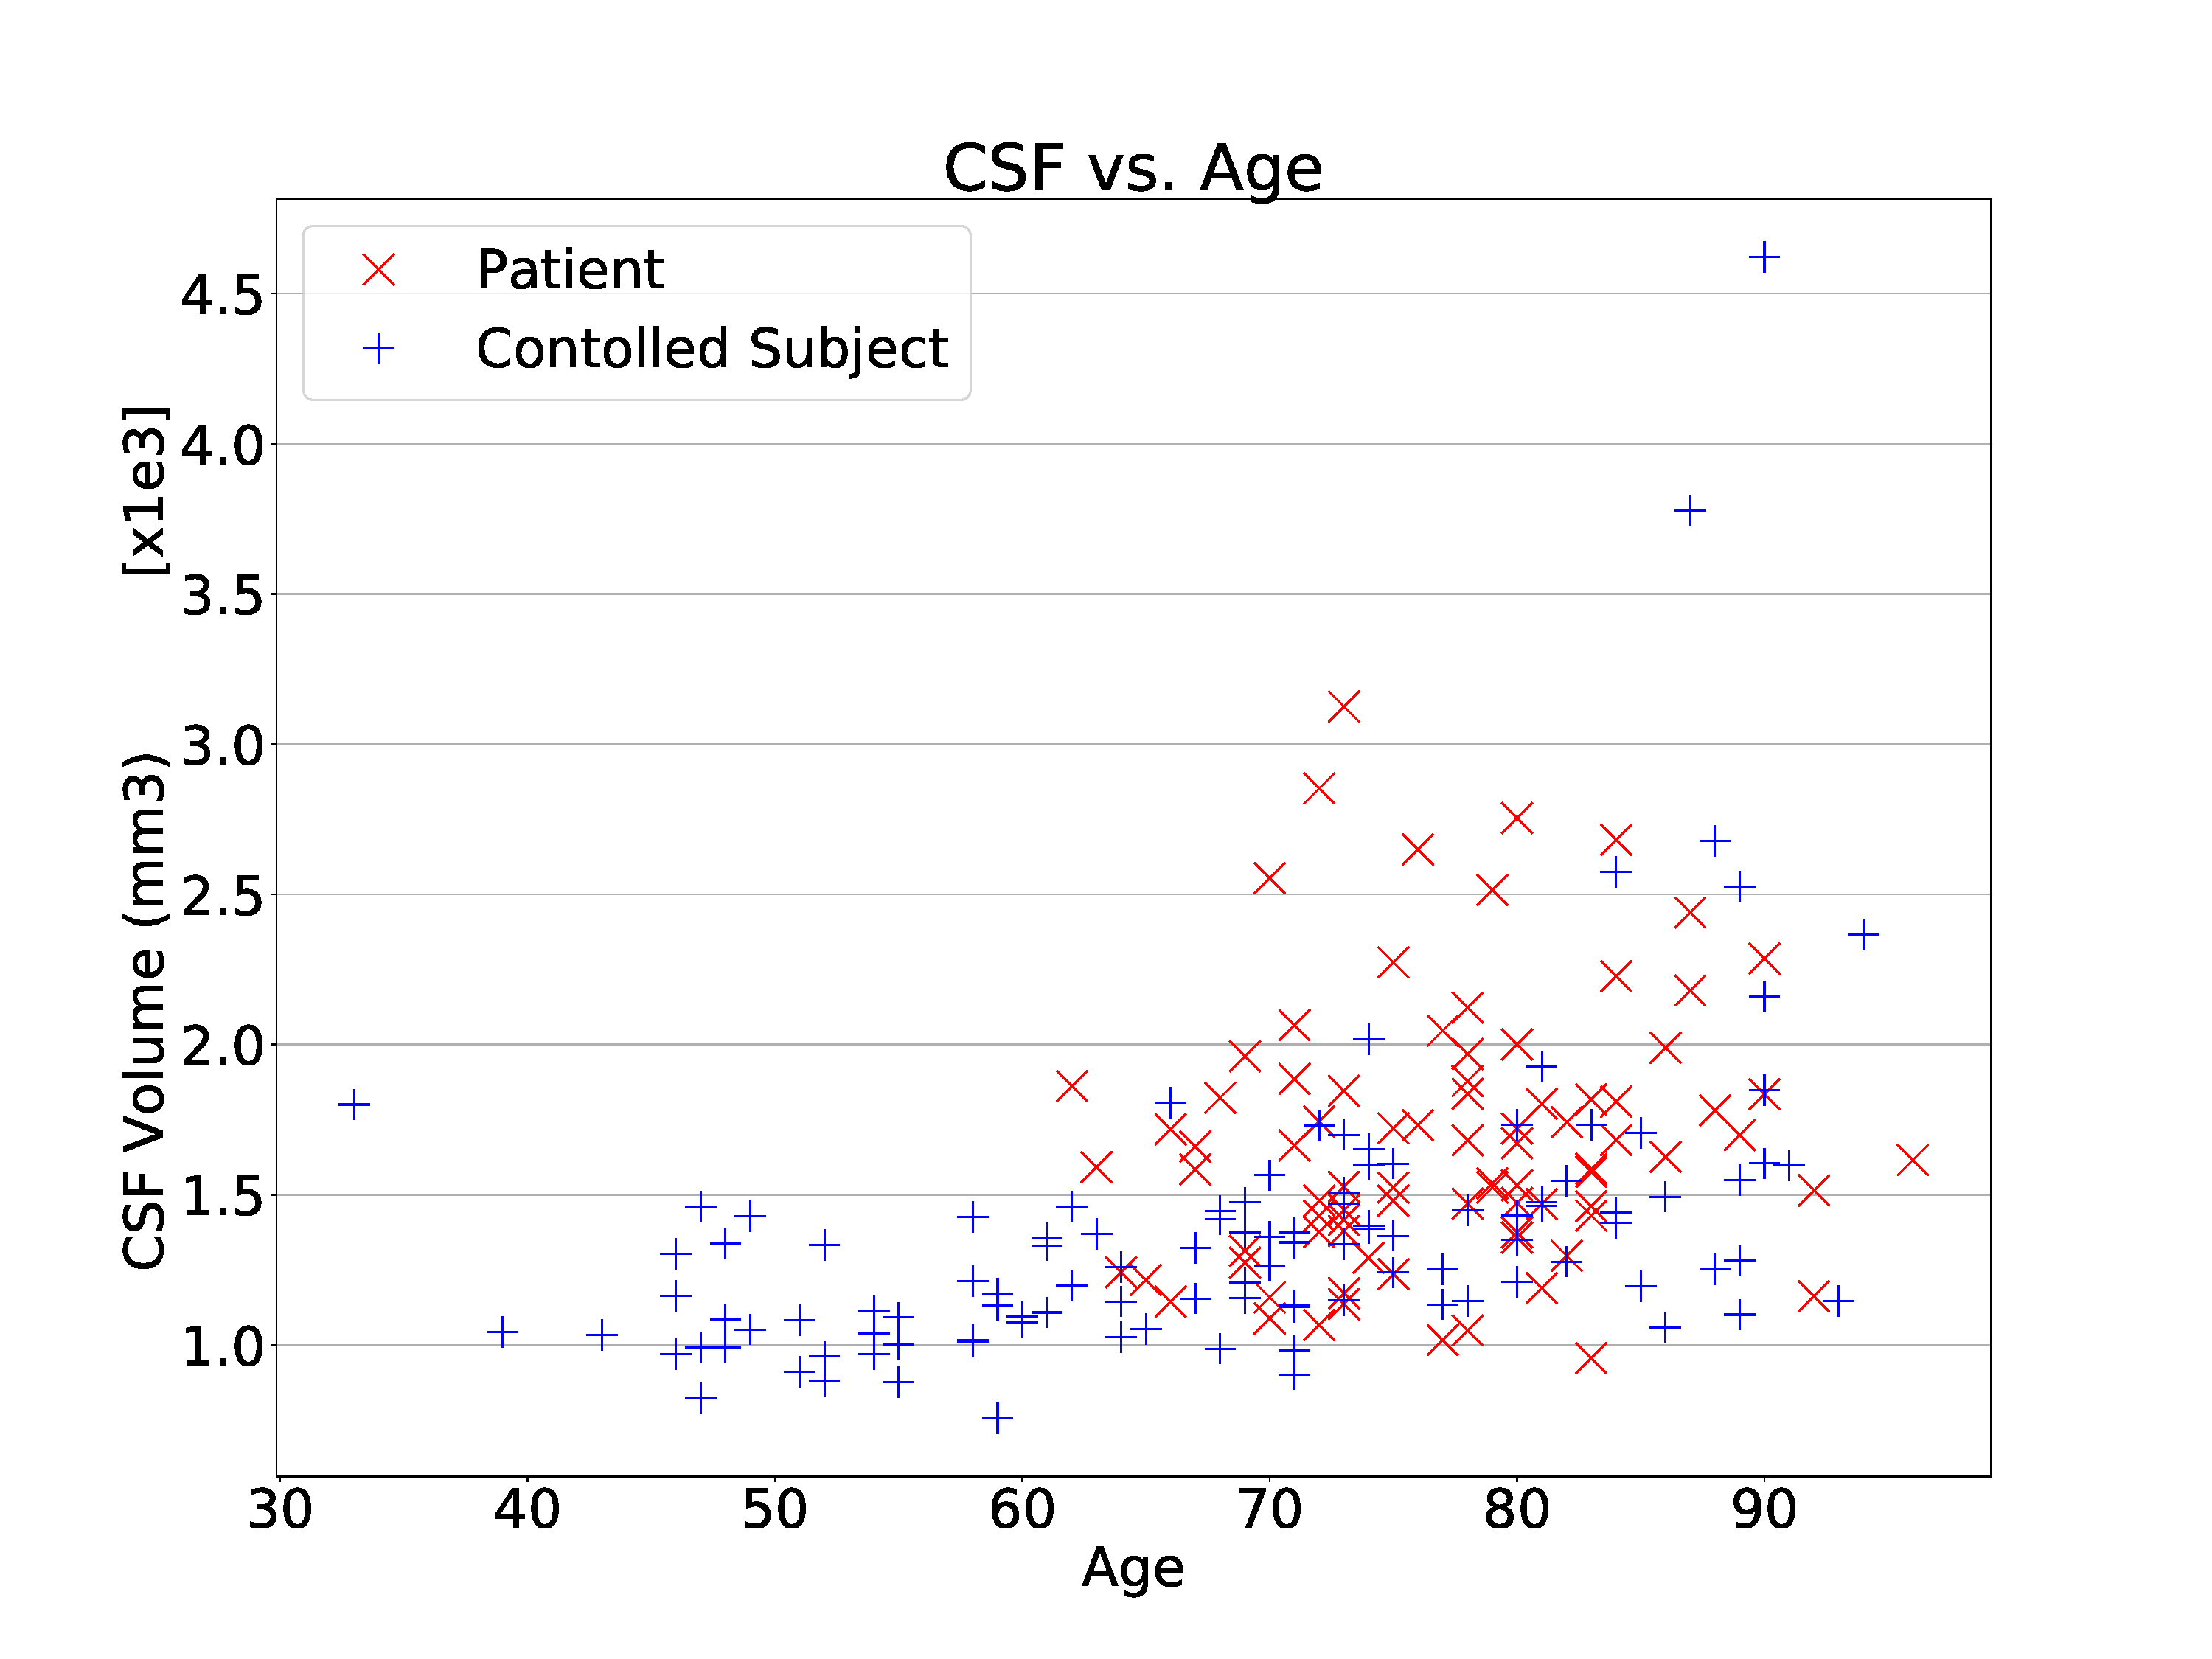
\includegraphics[width=\columnwidth]{images/AD-Age-CSF.pdf}
	\caption{CSF vs. age in AD patients and controlled subjects}
	\label{fig:AD-Age-CSF.pdf}
\end{figure}




\section{Algorithms and Techniques}
\label{sec:Alg}
Data Analysis is done using the following supervised machine learning Techniques:

\begin{itemize}
%	\item Naive Bayesian: No matter how strong the dependences among attributes are, naive Bayes can still be optimal if the dependences distribute evenly in classes, or if the dependences cancel each other out.
%	\item Decision Tree: The best feature of using trees for analytics is that it is easy to interpret and explain. To have a clear interpretation of data, we put decision tree in our selections as well. 
	\item Logistic Regression:
	Logistic regression deals with this problem by using a 
	logarithmic transformation on the outcome variable 
	which allow us to model a nonlinear association in a 
	linear way. Therefore, logistic regression is chosen here to evaluate linear classifiers in OASIS dataset classification task.
	
	\item Random Forests: Random Forests perform implicit feature selection and provide a pretty good indicator of feature importance. As the number of features are relatively high, using random forest can help us to try considering only important features.
	
	\item SVM: The kernel trick in SVM is to transform data and then based on these transformations, find an optimal boundary between the possible outputs. Simply, it does some extremely complex data transformations, then figures out how to separate data based on the labels or outputs defined. The benefit is that we can capture complex relationships between data points without having to perform difficult transformations on our own. The downside is that the training time is much longer as it is much more computationally intensive.
\end{itemize}


\subsection{Metrics}
Classifiers are commonly evaluated using either a numeric metric, such as accuracy, or a graphical representation of performance, such as a receiver operating characteristic (ROC) curve.

A very simple choice to evaluate learning algorithms is the score which is the percentage of passengers correctly predicted. This is known simply as "accuracy”.  Other metrics such as area under the curve (AUC), recall, and precision are also considered which can be obtained from confusion matrix and ROC curve. Here recall is an important metric as  it can be more detrimental to predict a patient is not sick if they are actually sick (False Negative), resulting in a decision
not to run further diagnostics and so causing serious complications from not treating the illness.

Two popular approaches for evaluating the performance of a classification algorithm on a data set are k-fold and leave-one-out cross validation. When the amount of data is large, k-fold cross validation should be employed to estimate the accuracy of the model induced from a classification algorithm, because the accuracy resulting from the training data of the model is generally too optimistic. Leave-one-out cross validation is a special case of k-fold cross validation, in which the number of folds equals the number of instances. When the number of instances either in a data set or for a class value is small, such as gene sequence data, leave-one-out cross validation should be adopted to obtain a reliable accuracy estimate for a classification algorithm. In this project as the number of instances is large enough, we study k-fold cross validation.

Then we apply statistical significant tests on the results obtained by k-fold cross validation. The following tests will be applied to compare different classifiers performance:

\begin{itemize}
	\item Student’s t-test (the simplest statistical test)
	\item Paired tests
\end{itemize}

\subsection{Implementation}

The three classifiers are implemented in \texttt{python} using \texttt{sklearn} library.


%
%\section{Visualization}
%Visualizations of graphs and data is done using \texttt{matplotlib} library.

%\subsection{Features Importance}
%Tree-based estimators can be used to compute feature importances, which in turn can be used to discard irrelevant features.
%
%Using feature importances with forests of trees, we can draw the importance of features to see if feature selection is necessary or not. The importance of features received from Random Forest model is shown in Figure.
%

\section{Expriments and Results}

The three algorithms mentioned in Section \ref{sec:Alg} are implemented to classify titanic dataset. The three algorithms are:
\begin{itemize}
	\item Logistic regression
	\item Random Forests
	\item SVM classification
\end{itemize}

\subsection{Hyperparameters tuning}
For each classifier there are parameters that needs to be tuned in order to have a fair comparison. The hyperparameters that are tuned here is as follows:
 
\begin{itemize}
	\item Logistic Regression
	\begin{itemize}
		\item Regularization Parameter
			\begin{itemize}
				\item \texttt{[1e-1, 1e-2, 1e-3, 1e-4, 1e-5]}
			\end{itemize}
		\item Tolerance
			\begin{itemize}
				\item \texttt{[1e-1, 1e-2, 1e-3, 1e-4, 1e-5]}
			\end{itemize}
	\end{itemize}

	\item Random Forests
		\begin{itemize}
			\item Number of estimators
			\begin{itemize}
				\item \texttt{5, 10, 15, 20, 25}
			\end{itemize}
			\item Max depth
			\begin{itemize}
				\item \texttt{[2-10]}
			\end{itemize}
		\end{itemize}
	\item SVM
		\begin{itemize}
			\item C (l2 Regularization Coefficient)
			\begin{itemize}
				\item \texttt{[0.1, 1, 10, 100, 1000]}
			\end{itemize}
			\item Gamma (Free parameter of the Gaussian radial basis function)
			\begin{itemize}
				\item \texttt{[10, 1, 1e-1, 1e-2, 1e-3, 1e-4]}
			\end{itemize}
		
		\item Kernel type
		\begin{itemize}
			\item \texttt{[Linear, Poly, rbf]}
		\end{itemize}
		\end{itemize}
\end{itemize}

\section{Results}
The algorithms were run over \texttt{199} samples with \texttt{139} features. Internal and external cross validation is applied with \texttt{K=10} for external and \texttt{k=5} for internal (parameter tunning cross validation).

The results for logistic regression, random forests, and SVM are shown in Tables \ref{tab:logit}, \ref{tab:rf}, and \ref{tab:svm}, respectively.

\begin{table*}
	\centering
	\caption{Logistic regression performance}
	\label{tab:logit}
	\csvautobooktabular{CSV/Logit.csv}
\end{table*}

\begin{table*}
	\centering
	\caption{Random forests performance}
	\label{tab:rf}
	\csvautobooktabular{CSV/RF.csv}
\end{table*}

\begin{table*}
	\centering
	\caption{Support Vector Machine performance}
	\label{tab:svm}
	\csvautobooktabular{CSV/SVM.csv}
\end{table*}


The metrics are as follows:
\begin{itemize}
	\item Accuracy
	\item Confusion matrix
	\begin{itemize}
		\item Recall
		\item Precision
	\end{itemize}
	\item AUC (Area Under ROC Curve)
\end{itemize}

After the metrics were obtained across the 10 outer folds, in order to determine whether there is a significant difference between the mean of the three algorithms, an Analysis of variance (ANOVA) test was performed for each of the metrics (accuracy, recall, precision, AUC). The null and alternate hypotheses are as follows:
\begin{itemize}
	\item \textbf{Null hypothesis}: The true mean of all the three algorithms are the same.
	\item \textbf{Alternate hypothesis}: The true mean of the three algorithms are different.
\end{itemize}

\subsection{ANOVA test}
 ANOVA provides a statistical test of whether or not the means of several groups are equal, and therefore generalizes the t-test to more than two groups. ANOVAs are useful for testing three or more means (groups or variables) for statistical significance.

The ANOVA test has an important assumption that must be satisfied in order for the associated p-value to be valid:
\begin{itemize}
	\item The population standard deviations of the groups are all equal. This property is known as homoscedasticity.
\end{itemize}

For that reason, we have to first calculate the standard deviation of the three groups of accuracy. The results are shown in Table

\begin{table}
	\centering
	\caption{Standard deviation on different criterions}
	\label{tab:std}
	\csvautobooktabular{CSV/std.csv}
\end{table}

As the standard deviation values are almost equal, we can perform ANOVA test. The results of ANOVA test is shown in Table

\begin{table}
	\centering
	\caption{ANOVA test on different criterions}
	\label{tab:anova}
	\csvautobooktabular{CSV/ANOVA.csv}
\end{table}

The ANOVA test results demonstrate that the three classifiers are not significantly different and the null hypothesis can not be rejected. If the ANOVA test on any of the metrics was almost less than 0.1, we could go further and perform t-test to detect statistically different pairs of classifiers. Nevertheless, we have performed Welch t-test in the next section to further prove that the classifiers are not significantly different.

\subsection{T-Test}
We calculate the T-test for the means of the pairs of two independent samples of scores, i.e. the scores obtained for algorithms.

The test measures whether the average (expected) value differs significantly across samples. If we observe a large p-value, for example larger than 0.05 or 0.1, then we cannot reject the null hypothesis of identical average scores. If the p-value is smaller than the threshold, e.g. 1\%, 5\% or 10\%, then we reject the null hypothesis of equal averages.

As Welch's t-test performs better than Student's t-test whenever sample sizes and variances are unequal between groups, and gives the same result when sample sizes and variances are equal, we use Welch's t-test. We also provide the results of and standard t-test. The results for both tests, Welch and standard t-test, are shown in Tables \ref{tab:welch} and \ref{tab:standard}, respectively. The results show the fact that when the variances are almost equal, Welch's t-test and standard t-test give similar results.

\begin{table*}
	\centering
	\caption{Welch t-test}
	\label{tab:welch}
	\csvautobooktabular{CSV/Welch-1.csv}
\end{table*}

\begin{table*}
	\centering
	\caption{Standard t-test}
	\label{tab:standard}
	\csvautobooktabular{CSV/Standard-1.csv}
\end{table*}

Considering the results of Welch's t-test, Table \ref{tab:welch}, we demonstrate that the null hypothesis cannot be rejected as the \texttt{p-value} is greater than 0.1 for any pair of algorithms and any metrics.

\section{Conclusion}
The results confirm that the volumetric measurements of different regions of the brain can be effectively used in AD identification. The experiments result also demonstrates that the original hypothesis that one of the algorithm chosen would not perform better than the other cannot be rejected through the experiments that have been done. In terms of the metrics chosen for comparison, the three algorithms performed similar, however it should be noted that the run time of SVM is significantly higher than the other two which is a benefit for logistic regression and random forests. The data preprocessing part also plays an important role in the quality of final results and accuracy. It may also affect the final results of classifier differently and therefore should be taken into account. As a result, Further work on preprocessing data can be considered as an important step in future work.

For future work, collecting more data of both controlled subjects and patients can help to achieve higher accuracy. Combining OASIS with Alzheimer’s Disease Neuroimaging Initiative (ADNI) dataset, which is another famous dataset in Alzheimer's disease, might help. Nevertheless, we should be aware of different scanning procedures and scaling as well as applying the same preprocessing and feature extraction on both dataset. Applying outliers detection can also be helpful, thereby detecting wrong labeled data to remove them from training set and finally, diagnosis accuracy improvement.



%------------------------------------------------





% \appendices
% \section{Proof of the First Zonklar Equation}
% Some text for the appendix.

% % use section* for acknowledgement
% \section*{Acknowledgment}


% The authors would like to thank...


% Can use something like this to put references on a page
% by themselves when using endfloat and the captionsoff option.

%----------------------------------------------------------------------------------------
%	BIBLIOGRAPHY
%----------------------------------------------------------------------------------------
\bibliographystyle{unsrt}
\bibliography{ref}

\end{document}


